\documentclass[AMA,Times1COL]{WileyNJDv5} %STIX1COL,STIX2COL,STIXSMALL

\articletype{Article Type}%

\received{Date Month Year}
\revised{Date Month Year}
\accepted{Date Month Year}
\journal{Journal}
\volume{00}
\copyyear{2023}
\startpage{1}

\raggedbottom

\begin{document}

\title{Functional Mixed-Effect Modeling of Multivariate Jaw Kinematics}

\author[1]{Palmer Swanson}

\author[2,3]{Author Two}

\author[3]{Author Three}

\authormark{SWANSON \textsc{et al.}}
\titlemark{Functional Mixed-Effect Modeling of Multivariate Jaw Kinematics}

\address[1]{\orgdiv{Depertment of Statistics}, \orgname{Florida State University}, \orgaddress{\state{Florida}, \country{United States of America}}}

\address[2]{\orgdiv{Department Name}, \orgname{Institution Name}, \orgaddress{\state{State Name}, \country{Country Name}}}

\address[3]{\orgdiv{Department Name}, \orgname{Institution Name}, \orgaddress{\state{State Name}, \country{Country Name}}}

\corres{Corresponding author Palmer Swanson, 
Department of Statistics, Florida State University 214 Rogers Building (OSB), 117 N. Woodward Ave. P.O. Box 3064330, Tallahassee, FL 32306-4330
 \email{pjswanson@fsu.edu}}

\presentaddress{This is sample for present address text this is sample for present address text.}

%\fundingInfo{Text}
%\JELinfo{ejlje}

\abstract[Abstract]{Temporomandibular joint (TMJ) disorders affect up to one-third of adults and are associated with pain, joint clicking, and compromised jaw function, significantly impacting quality of life. Understanding how individual-level characteristics influence jaw motion is therefore of clinical interest. In this work, we model three-dimensional jaw kinematic data using a Bayesian function-on-scalar regression framework. The data consist of tri-variate functional outcomes for 40 participants across multiple tasks, with motion tracked at key anatomical points on the jaw.

    We extend prior work by Goldsmith to develop a hierarchical spline-based model for tri-variate functional data that accounts for subject-specific random effects and fixed covariates. To address computational challenges associated with high-dimensional covariance estimation in multivariate models, we propose a modified version of the model that avoids large inverse-Wishart priors at the level-1 error, instead shifting covariance structure into the random effects. We compare performance using a Gibbs sampler and a Hamiltonian Monte Carlo (HMC) implementation in STAN.

    Simulation studies evaluate both methods across varying numbers of covariates, knots, and noise levels. Results suggest that while the Gibbs sampler generally achieves higher posterior coverage and lower IMSE, the STAN implementation achieves substantially faster computation times. We apply the model to real jaw tracking data, finding that demographic and clinical covariates significantly influence jaw motion. }

\keywords{Bayesian Regression, Trivariate Data, Functional Response, Kinematic Data, Gibbs Sampler, Hamiltonian Monte Carlo}

\jnlcitation{\cname{%
\author{Swanson P},
\author{Lauritzen P},
\author{Erath C}, and
\author{Mittal R}}.
\ctitle{Functional Mixed-Effect Modeling of Multivariate Jaw Kinematics} \cjournal{\it J Comput Phys.} \cvol{2021;00(00):1--18}.}


\maketitle

%\renewcommand\thefootnote{}
%\footnotetext{\textbf{Abbreviations:} ANA, anti-nuclear antibodies; APC, antigen-presenting cells; IRF, interferon regulatory factor.}

%\renewcommand\thefootnote{\fnsymbol{footnote}}
%\setcounter{footnote}{1}

\section{Introduction}\label{sec1}

For humans, the face plays a crucial role in identification, communication, and proper functioning of certain senses.  The jaw plays a jointly important role in these activities, as well as mastication and communication.  Unfortunately, many people - up to a third of adults - suffer from dysfunction of the temporomandibular joint, also known as TMJ disorders\cite{buescher_temporomandibular_2007}.  Symptoms of TMJ disorders commonly include pain, clicking of the jaw joint, dislocation of the jaw, headaches, and dizziness.  Any one of these can greatly reduce the quality of life of an individual.  For that reason, it is important to better understand the impact of various covariates on human jaw movement.  

This work focuses on modeling the three-dimensional kinematic motion of various regions of the jaw, with particular attention to how this motion is influenced by scalar covariates.  The motivating data set for this study involved three-dimensional kinematic data of subjects' jaws at various positions and for various oral tasks.  Each subject was fitted with small sensors on their central incisor, left condylar apex, and right condylar apex.  Subjects completed repeated open-close, lateral left, lateral right, and anterior/posterior shift tasks.  Our data consisted of 776 three-dimensional function observations for 40 subjects (25 males and 25 females), across the four tasks.  

Kinematic data is obtained for each repeated task.  In other words, we have observed X, Y, and Z motion data for each subject, repetition, and task.  In other words, we are provided tri-variate functional outcomes \(P_{ijk}^X(t), P_{ijk}^Y(t), P_{ijk}^Z(t)\) for subject \(i\), repetition \(j\), and task \(k\).  Fig. 1 provides and example of the observed data.  The data is facetted into each Cartesian coordinate, and trajectories are grouped together by subject.  

The goal of this analysis is to understand the impact of multiple different covariates such as age, sex, and other demographic/clinical variables on three-dimensional kinematic motion, while incorporating subject specific random effects. 

%\section{Description of 3D Kinematic Data}\label{sec2}
\subsection{Description of 3D Kinematic Data}

A description of the motivating dataset, its structure, and means of collection is appropiate at this point.  The study population in this work consists of 40 subjects recruited to XXX institute.  

Each subject is fitted with several markers on several parts of the jaw: the lower central incisor as well as the left and right apex of the mandible.  Subjects were then instructed to perform various tasks, including opening and closing the mandible, moving the mandible to the left and back, and moving the mandible to the right and back.  Describe the data process more.

For each subject and task, numerous replications are run and three dimensional kinematic data in cartersian coordinates relative to the starting position are recorded; for each task, the X, Y, and Z coordinates of jaw movement are observed.  In other words, we are provided tri-variate functional outcomes \(P_{ijk}^X(t), P_{ijk}^Y(t), P_{ijk}^Z(t)\) for subject \(i\), repetition \(j\), and task \(k\).  An example set of data is provided below:

\begin{figure}[h]
    \centering
    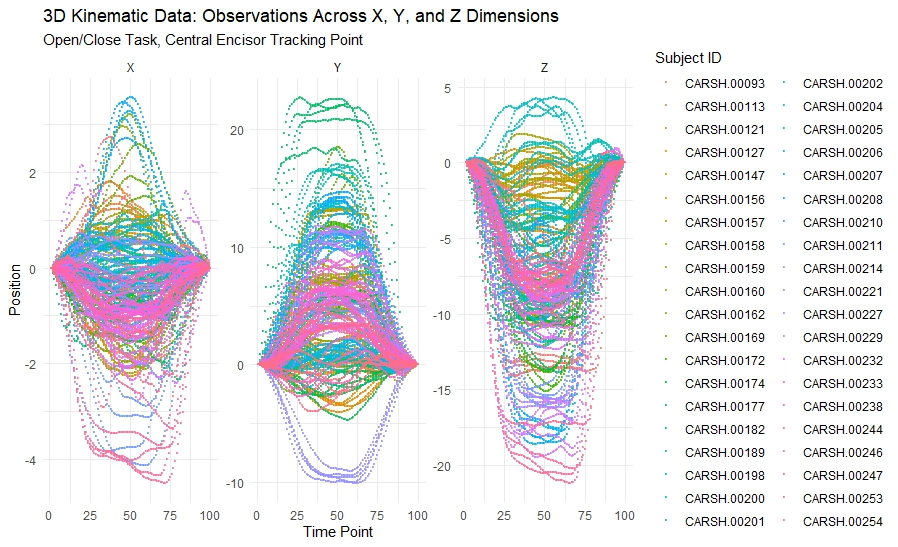
\includegraphics[width = 0.7\textwidth]{OC_CI_raw.jpeg}
    \caption{Observed Kinematic Data for the Central Encisor Tracking Point, Open/Close Task}
    \label{fig:example_dat}
\end{figure}

\subsection{Description of Covariates}
In addition to kinematic data on each subjects tasks and replications, we also have data on baseline scalar covariates.  Baseline scalar covariates consisted of sex, age, ethnicity, skeletal classification, and the presence of TMD symptoms. Age was modeled as a continuous predictor, while the remaining covariates were categorical.  A summary of baseline covariates is provided in Table \ref{description}.  The "average" subject was a 32 year old caucasian female with a class 3 skeletal type and no TMD symptoms.  When creating the fixed effect design matrix, the categorical variables are encoded via dummy variables.  

%\subsection{Methods}
\section{Methods and Background}\label{sec2}

It is helpful to consisder this problem from the point of view that we have functional data for a group of subjects and replications.

In traditional statistical analysis, data often consists of scalar values, meaning individual numerical measurements.  Classical statistical methods, such as regression models, hypothesis testing, and probability distributions, are well-suited for analyzing this type of data.  However, in many real-world applications, data is not limited to scalar observations. Instead, it can take the form of curves or functions observed over a continuum, such as time or space. Functional data of this nature appears in numerous disciplines. For instance, growth curves are frequently analyzed in biological and medical research to study changes in body measurements over time \cite{rao_statistical_1958}.  Similarly, hormone levels fluctuate within an individual’s body throughout the day, and their trajectories provide insights into biological processes \cite{brumback_smoothing_1998}. In engineering and environmental sciences, sensor data often consists of time series that capture continuous readings of temperature, pressure, or other physical phenomena \cite{nikolova_curve_2009}. Even in finance, stock prices evolve over time as continuous functions, and understanding their dynamics is critical for optomizing investment strategies\cite{fama_behavior_1965}.  In other words, data often presents itself as curves, functions, or other not scalar manifestations.  

There are a variety of methods for analysis with functional data depending on if the response, predictors, or both are functional.  One of the early attempts at doing so was the 1982 paper by Ramsay\cite{ramsay_when_1982}.  The focus of this work is the scenario where the response is functional and we are attempting to understand the connection between scalar predictors and said functional outcome.  This scenario is commonly referred to as function-on-scalar (FOS) regression.  Ramsay and Silverman\cite{ramsay_functional_2005} introduced a basic model for FOS regression that took the form of:

\begin{equation}
    \boldsymbol{y}\left(t\right) = \boldsymbol{Z}\boldsymbol{\beta}\left(t\right) + \boldsymbol{\epsilon}\left(t\right)
\end{equation}

Typically, the observed data \(\boldsymbol{y}\left(t\right)\) is not functional in observation.  Rather, we assume that the observed data is simply a realization of the true response curves as time points \(t_1, \dots,t_n\)\cite{reiss_fast_2010}.  This introduces an inherent issue of dimensionality: while the true response is theoretically infinite-dimensional, we must develop models that approximate it using a finite number of parameters.  Fortunately, there are several ways to do this, including Fourier series, wavelets, principal components, and the focus of this work, spines\cite{morris_functional_2015}.  The use of splines also allows for the incorporation of penalty terms, which can help control overfitting and improve generalisabilty.

There are extensive pools of literature to pull from with respect to functional data analysis and function on scalar regression in particular.  Beginning in the 1950's, prinicpal components were used to model the mean of curves.  

\subsection{Goldsmith's Univiariate Model}
This work is motivated by the model elucidated by Goldsmith.  Therefore a brief description of the "base" model is appropiate.  We observe functional data, at this stage univariate, for each subject, collected over multiple visits, resulting in a total number of observations \(n\) across all subjects.  This data consist of curves representing possibily multiple dimensions of positions tracked over time, along with a set of scalar covariates for each subject.  Goldsmith's as well as our model includes fixed effects to capture the influence of these covariates, subject-specific random effects to account for individual differences, and residual curves that may be correlated.  We and Goldsmith estimate these effects using penalized splines, specifically cubic B-splines with a penalty that controls smoothness

Goldsmith assumes that the data is comprised of functional responses and scalar covariates for subjects \(i=1,\dots, I\) and visists \(j=1,\dots, J_i\), meaning that we have \(n = \sum_{i}J_i\) total observations.  He formulates a model with functional responses observed on a uniform grid of length \(D\) for all subjects and visists, giving the following model:

\begin{equation}
    \boldsymbol{y}_{ij} = \boldsymbol{\omega}_i\boldsymbol{\beta} + \boldsymbol{z}_{ij}\boldsymbol{b} + \boldsymbol{\epsilon}_{ij}
\end{equation}

where \(\boldsymbol{y_{ij}}\) denotes a \(1 \times D\) functional outcome vector for subject \(\emph{i}\) and replication \(\emph{j}\), \(\boldsymbol{\omega_i}\) denotes a fixed effect design vector, \(\boldsymbol{z_i}\) denotes a random effects design vector, \(\boldsymbol{\beta}\) denotes the fixed effect functional coefficient matrix, \(\boldsymbol{b}\) denotes the random effect coefficient matrix, and  \(\boldsymbol{\epsilon}_{ij}\) denotes a \(1 \times D \) residual vector following a multivariate normal distribution centered at 0\cite{goldsmith_assessing_2016}

\(\boldsymbol{\beta}\) and \(\boldsymbol{b}\) are expanded via splines.  A spline matrix \(\Theta\) is created of size \(D \times K\), where \(K\) is the number of basis functions used.  Correspondingly, matrices of spline coefficients are introduced, meaning that \(\boldsymbol{\beta}\) and \(\boldsymbol{b}\) are rewritten as \(\left[\Theta B_w\right]^T\) and \(\left[\Theta B_Z\right]^T\) respectively.

The columns of \(B_w\) and \(B_Z\) are penalized with a penalty matrix \(P\) that is selected \emph{a priori}.  Variances in \(B_w\) are unqiue to each coefficient, whereas the variances in the random effects are pooled.  This gives Goldsmith the following model for the univariate case:

\begin{equation}
    \begin{split}
        \boldsymbol{y}_{ij} = \boldsymbol{\omega}_iB_W^T\Theta^T + \boldsymbol{z}_{ij}B_Z^T\Theta^T + \boldsymbol{\epsilon}_{ij}\\
        \boldsymbol{\epsilon}_{ij} \sim N[0, \Sigma]\\
        B_{Z,i} \sim N[0, \sigma_z^2P^{-1}]\quad \text{for} \quad i = 1,\dots, I\\
        B_{W, k} \sim N[0, \sigma_{W,k}^2P^{-1}]\quad \text{for} \quad k = 0,\dots, p\\
    \end{split}
\end{equation}

By placing an inverse Wishart prior on \(\boldsymbol{\epsilon}_{ij}\),  inverse gamma priors on the variance terms, and recentering the model, Goldsmith presents the following:

\begin{equation}
    \begin{split}
        Y = ZB_Z^T\Theta^T + \epsilon\\
        \epsilon\sim N[0, \Sigma\otimes I_n]\\
        \Sigma \sim IW[v, \Psi]\\
        B_{Z,i} \sim N[B_w \boldsymbol{w}_i^T, \sigma_z^2P^{-1}]\quad \text{for} \quad i = 1,\dots, I\\
        \sigma_z^2 \sim IG[a_z, b_z]\\
        B_{W, k} \sim N[0, \sigma_{W,k}^2P^{-1}]\\
        \sigma_{W,k}^2 \sim IG[a_{W,k}, b_{W,k}]\quad \text{for} \quad k = 1,\dots, p
    \end{split}
\end{equation}

In the paper, he provides derivations to obtain conditional distributions for model parameters and uses these to impliment a Gibbs sampler.  

\subsection{Higher Dimensions}
Goldsmith provides a model for bivariate data; his motivating dataset is bivariate in nature (hand movement).  He provides a model for two dimensions\cite{goldsmith_assessing_2016}.  He concatenates data and spline coefficient matrices.  Specifically, \(Y = [Y_1,Y_2, Y_3]\), where \(Y_i, i\in(1,2)\) corresponds to functional outcomes in the X and Ydimensions, \(B_W^T = [B_{1,W}^T, B_{2,W}^T]\), corresponding to the fixed effect spline coefficients in two dimensions, and \(B_Z^T = [B_{1,Z}^T, B_{2,Z}^T]\) corresponding to the random effect spline coefficients in two dimensions.  Taking advantage of Kronecker product structure,  Goldsmith writes out the following model:

\begin{equation}
    \begin{split}
        Y = ZB_Z^T\left(I_2 \otimes\Theta^T\right) + \epsilon\\
        \epsilon\sim N[0, \Sigma\otimes I_n]\\
        \Sigma \sim IW[v, \Psi]\\
        B_{Z,i} \sim N[B_w \boldsymbol{w}_i^T, \text{diag}\left(\sigma_{1,Z}^2, \sigma_{2,Z}^2\right)\otimes P^{-1}]\quad \text{for} \quad i = 1,\dots, I\\
        \sigma_{m,Z}^2 \sim IG[a_{m,Z}, b_{m,Z}]\quad \text{for} \quad m = 1,2\\
        B_{W,i} \sim N[0, \text{diag}\left(\sigma_{1,W_{k}}^2, \sigma_{2,W_{k}}^2\right)\otimes P^{-1}]\\
        \sigma_{m,W_{k}}^2 \sim IG[a_{m,W_{k]}}, b_{m,W_{k}}]\quad \text{for} \quad m = 1,2 \quad\text{and} \quad k = 1,\dots, p
    \end{split}
\end{equation}

In this model, the fixed and random effects for each dimension are assumed independent and penalized separately.  The uni-variate Gibbs sampler is easily adapted to the two dimensional case.  

\subsection{Note on Penalty Matrix \(P\)}

In Goldsmith, the penalty matrix \(P\) is constructed by using \(\alpha  P_{0} + (1 - \alpha) P_{2} \), where \(P_{0}\) is the identity matrix and \(P_{2}\) is the second derivative penalty matrix.  This weighted sum is implemented to alleviate the nonivertability of \(P_{2}\).  Goldsmith suggests setting \(\alpha\) to be small, less than 0.01 in order to avoid enforcing shrinkage.  In general, I concur with this heuristic, though I would caution against setting \(\alpha\) to be \emph{too} small.  The reason for this is that the magnitude of the smallest eigenvalue of the resulting \(P\) matrix move linearly with \(\alpha\); if \(\alpha\) is too small, then the smallest eigenvalue could be numerically/computationally 0, making \(P\) almost non-invertible.  

\subsection{Working Models}
In this section, we describe two potential working models for the analysis of tri-variate (three-dimensional) functional data, extending the bivariate framework of Goldsmith \cite{goldsmith_assessing_2016}. Our goal is to provide a flexible modeling structure while addressing computational and statistical challenges posed by high-dimensional covariance estimation.

\subsubsection{Goldsmith's Extended Model}
As mentioned earlier, Goldsmtih laid out a model for bivariate data.   For the extension to three dimensions, we continue to follow his lead, giving the following model for three dimensional functional data:

\begin{equation}
    \begin{split}
        Y = ZB_Z^T\left(I_3 \otimes\Theta^T\right) + \epsilon\\
        \epsilon\sim N[0, \Sigma\otimes I_n]\\
        \Sigma \sim IW[v, \Psi]\\
        B_{Z,i} \sim N[B_w \boldsymbol{w}_i^T, \text{diag}\left(\sigma_{1,Z}^2, \sigma_{2,Z}^2, \sigma_{2,Z}^3\right)\otimes P^{-1}]\quad \text{for} \quad i = 1,\dots, I\\
        \sigma_{m,Z}^2 \sim IG[a_{m,Z}, b_{m,Z}]\quad \text{for} \quad m = 1,2, 3\\
        B_{W,i} \sim N[0, \text{diag}\left(\sigma_{1,W_{k}}^2, \sigma_{2,W_{k}}^2, \sigma_{3,W_{k}}^2\right)\otimes P^{-1}]\\
        \sigma_{m,W_{k}}^2 \sim IG[a_{m,W_{k]}}, b_{m,W_{k}}]\quad \text{for} \quad m = 1,2, 3 \quad\text{and} \quad k = 1,\dots, p
    \end{split}
\end{equation}

\subsubsection{Alternative Model}
In his model, Goldsmith places an inverse-Wishart prior on the level 1 covariance structure.  There is one cause for concern with this: for observations in three dimensions with each dimension being observed across a grid of \(D\), the level 1 covariance matrix would have to be \(3*D\times 3*D\).  In the case of \(D=100\), that would mean that our level 1 covariance matrix would be \(300\times300\).  As the dimensionality of the matrix involved increases, the scale parameter also must increase to for the distribution to remain proper.  A result of this is that the Inverse Wishart \(IW\left(n\boldsymbol{S} + \Psi, n + v\right)\) posterior distribution tends to concentrate more tightly around its prior expected value: \(\Psi/{\left(v-p-1\right)}\)\cite{zhang_note_2021}. When the scale matrix is the identity matrix, this expected value is proportional to the identity matrix itself; using an Inverse Wishart prior with an identity scale matrix can lead to over-shrinkage of the estimated covariance matrix towards the identity matrix.

In addition, we endeavor to use STAN, which encounters computational difficulties for high dimensional inverse wishart distributions.  To this end, we propose a slightly modified model that still accounts for correlation will not needing to delve into the uncertainty of higher order inverse Wishart distributions: 

\begin{equation}
    \begin{split}
    Y = ZB_Z^T\left(I_3 \otimes\Theta^T\right) + \epsilon\\
    \epsilon\sim N[0, \sigma_{0}^2 I_n]\\
    B_{Z,i} \sim N[B_w \boldsymbol{w}_i^T, \Omega_Z\otimes P^{-1}]\quad \text{for} \quad i = 1,\dots, I\\
    \Omega_Z \sim IW [v_z, \Psi_z]\\
    B_{W,i} \sim N[0, \Omega_{W,k}\otimes P^{-1}]\\
    \Omega_{W,k} \sim IW[v_{w,k}\Psi_{w,k}]\quad\text{for} \quad k = 1,\dots, p
    \end{split}
\end{equation}

In other words, we have moved the dependence from the level 1 error structure into the fixed and random effects.  The intuiton behind this is that now, rather than a \(300\times 300\) covariance matrix, out model only has several \(3\times 3\).  The intutiton to this approach is that not only is the computational burden reduced, but the mixing in MCMC sampling (especially in STAN) is also improved.  Furthermore, this also allows for more interpretable covariance structures at the subject and covariate levels.  This setup allows for data borrowing across dimensions without forcing the residual error covariance to absorb all variation.  

\section{Simulation}\label{sec3}
In statistics, simulation studies are often used; they can offer emperical evidence of a new method.  Additionally the controlled enviroment under which they are run allows for easy measurement of accuracy and repeatability.  This work is no different.  We demonstrate the performance of these two competing models by simulating three dimensional kinematic data.  Code required to reproduce these data generation and simulation steps may be found at:XXX.  

\subsection{Data Generation}
In general, the generated data is generated assuming a grid length \(D = 25\) in all three dimensions for a total grid length of 75.  The data follows a model structured in the following fashion:

\begin{equation}
    \underbrace{Y_{gen}}_{n\times 3D} = \underbrace{\underbrace{X}_{n\times p}*\underbrace{\beta}_{p\times 3D}}_{n\times 3D} + \underbrace{\underbrace{Z}_{n\times I}*\underbrace{b}_{I\times 3D}}_{n\times 3D} + \underbrace{\epsilon}_{n\times 3D}
\end{equation}

We generate smooth functional coefficients using B-splines for three-dimensional data. In doing so, we create a coefficient matrix for each dimension (X, Y, and Z) by applying a B-spline basis and random coefficients.  This leaves us with a \(p\times 3*D\) grid of coefficients, where each block corresponds to smooth coefficients functions in each dimension.  The subject design matrix \(X\) is generated from a normal distribution with a user specified variance.  

To obtain the fixed effect components of this data, we generate an \(n\times p\) design matrix comprised of baseline covariates for each of the \(I\) subjects over \(J_i\) replications and multiply this by the matrix containing the grid of coefficients.  For subject specific random effects, an \(n\times I\) design matrix is generated and multiplied by random coefficients generated from a standard normal distribution.  To generate level-1 errors, we draw \(n\times 3*D\) values from a standard normal distribution. 

An example of this simulated data is shown below:

\begin{figure}[h]
    \centering
    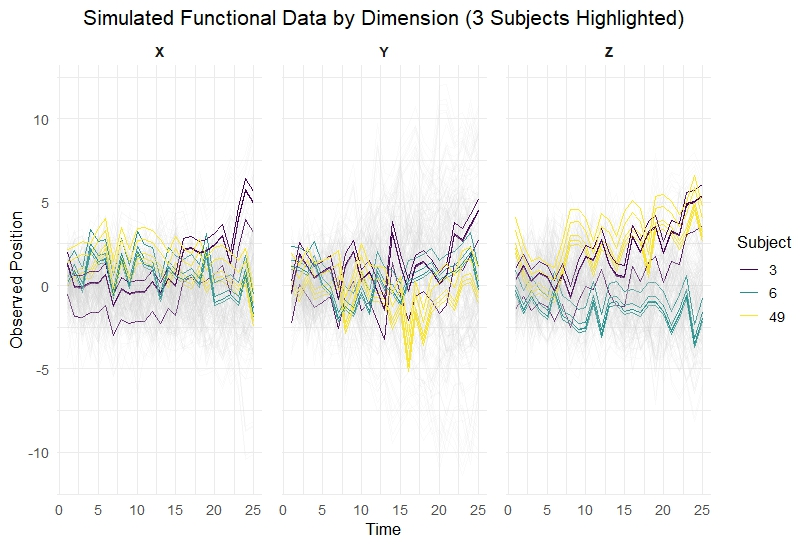
\includegraphics[width = 0.7\textwidth]{simulated_dat.jpeg}
    \caption{Example of Simulated Data}
    \label{fig:sim_dat}
\end{figure}

\subsection{Results}
In our simulation, we varied several key components of the model: the number of knots used in data estimation, the number of covariates, and the variance of both fixed and random effect variances, using both the STAN code and comparing the results to Goldsmith's tri-variate Gibbs sampler.  For the STAN model, we ran four parallel chains, each chain containing 2000 iterations (1000) burn in, for a total of 8000 iterations with the first 4000 discarded as burnin.  The for the tri-variate Goldsmith sampler, one chain with 8000 iterations and 4000 burn in iterations were run to have analysis be roughly comparable.    

Goldsmith's model spent a considerable amount of time discussing various initial values and hyperparameter values.  In particular he discusses an initial value for the inverse Wiwshart Scale parameter.  As our model does away with most of those initial values, we did not set initial values and largely used uninformative diagonal matrices as initial scale parameters for our smaller inverse Wishart distribution.

For each condition, 10 datasets were generated and both the Gibbs and STAN samplers were run, and several measures of performance were recorded including computation time (in seconds), integrated mean squared error (compared to the "true" coefficient curves), and mean coverage across all coefficient curves.  The results are shown in Table~\ref{tab:simulation_results}.  

In terms of coverage, both the STAN model and the Gibbs sampler model oftein acheive coverage \(>\) 90\%.  For some cases however, STAN coverage fell to 79.8\%.  The two models had comparable IMSE values.  In terms of computation time, Gibbs sampling was consistently much slower than STAN, occasionally by an order of magnitude.  Increasing the number of knots in the fitted model often improved coverage and reduced IMSE.  

\section{Emperical Results}
Now, we turn our attention to the emperical data described earlier.  The focus in on the estimation of the the significance of several scalar covariates on the overall three dimensional kinematic motion of the jaw.  The categorical variables are encoded as dummy variables for the purposes of design matrices.  We used the modified Gibbs sampler with one chain.  Below are some results from this: 

\begin{figure}[h]
    \centering
    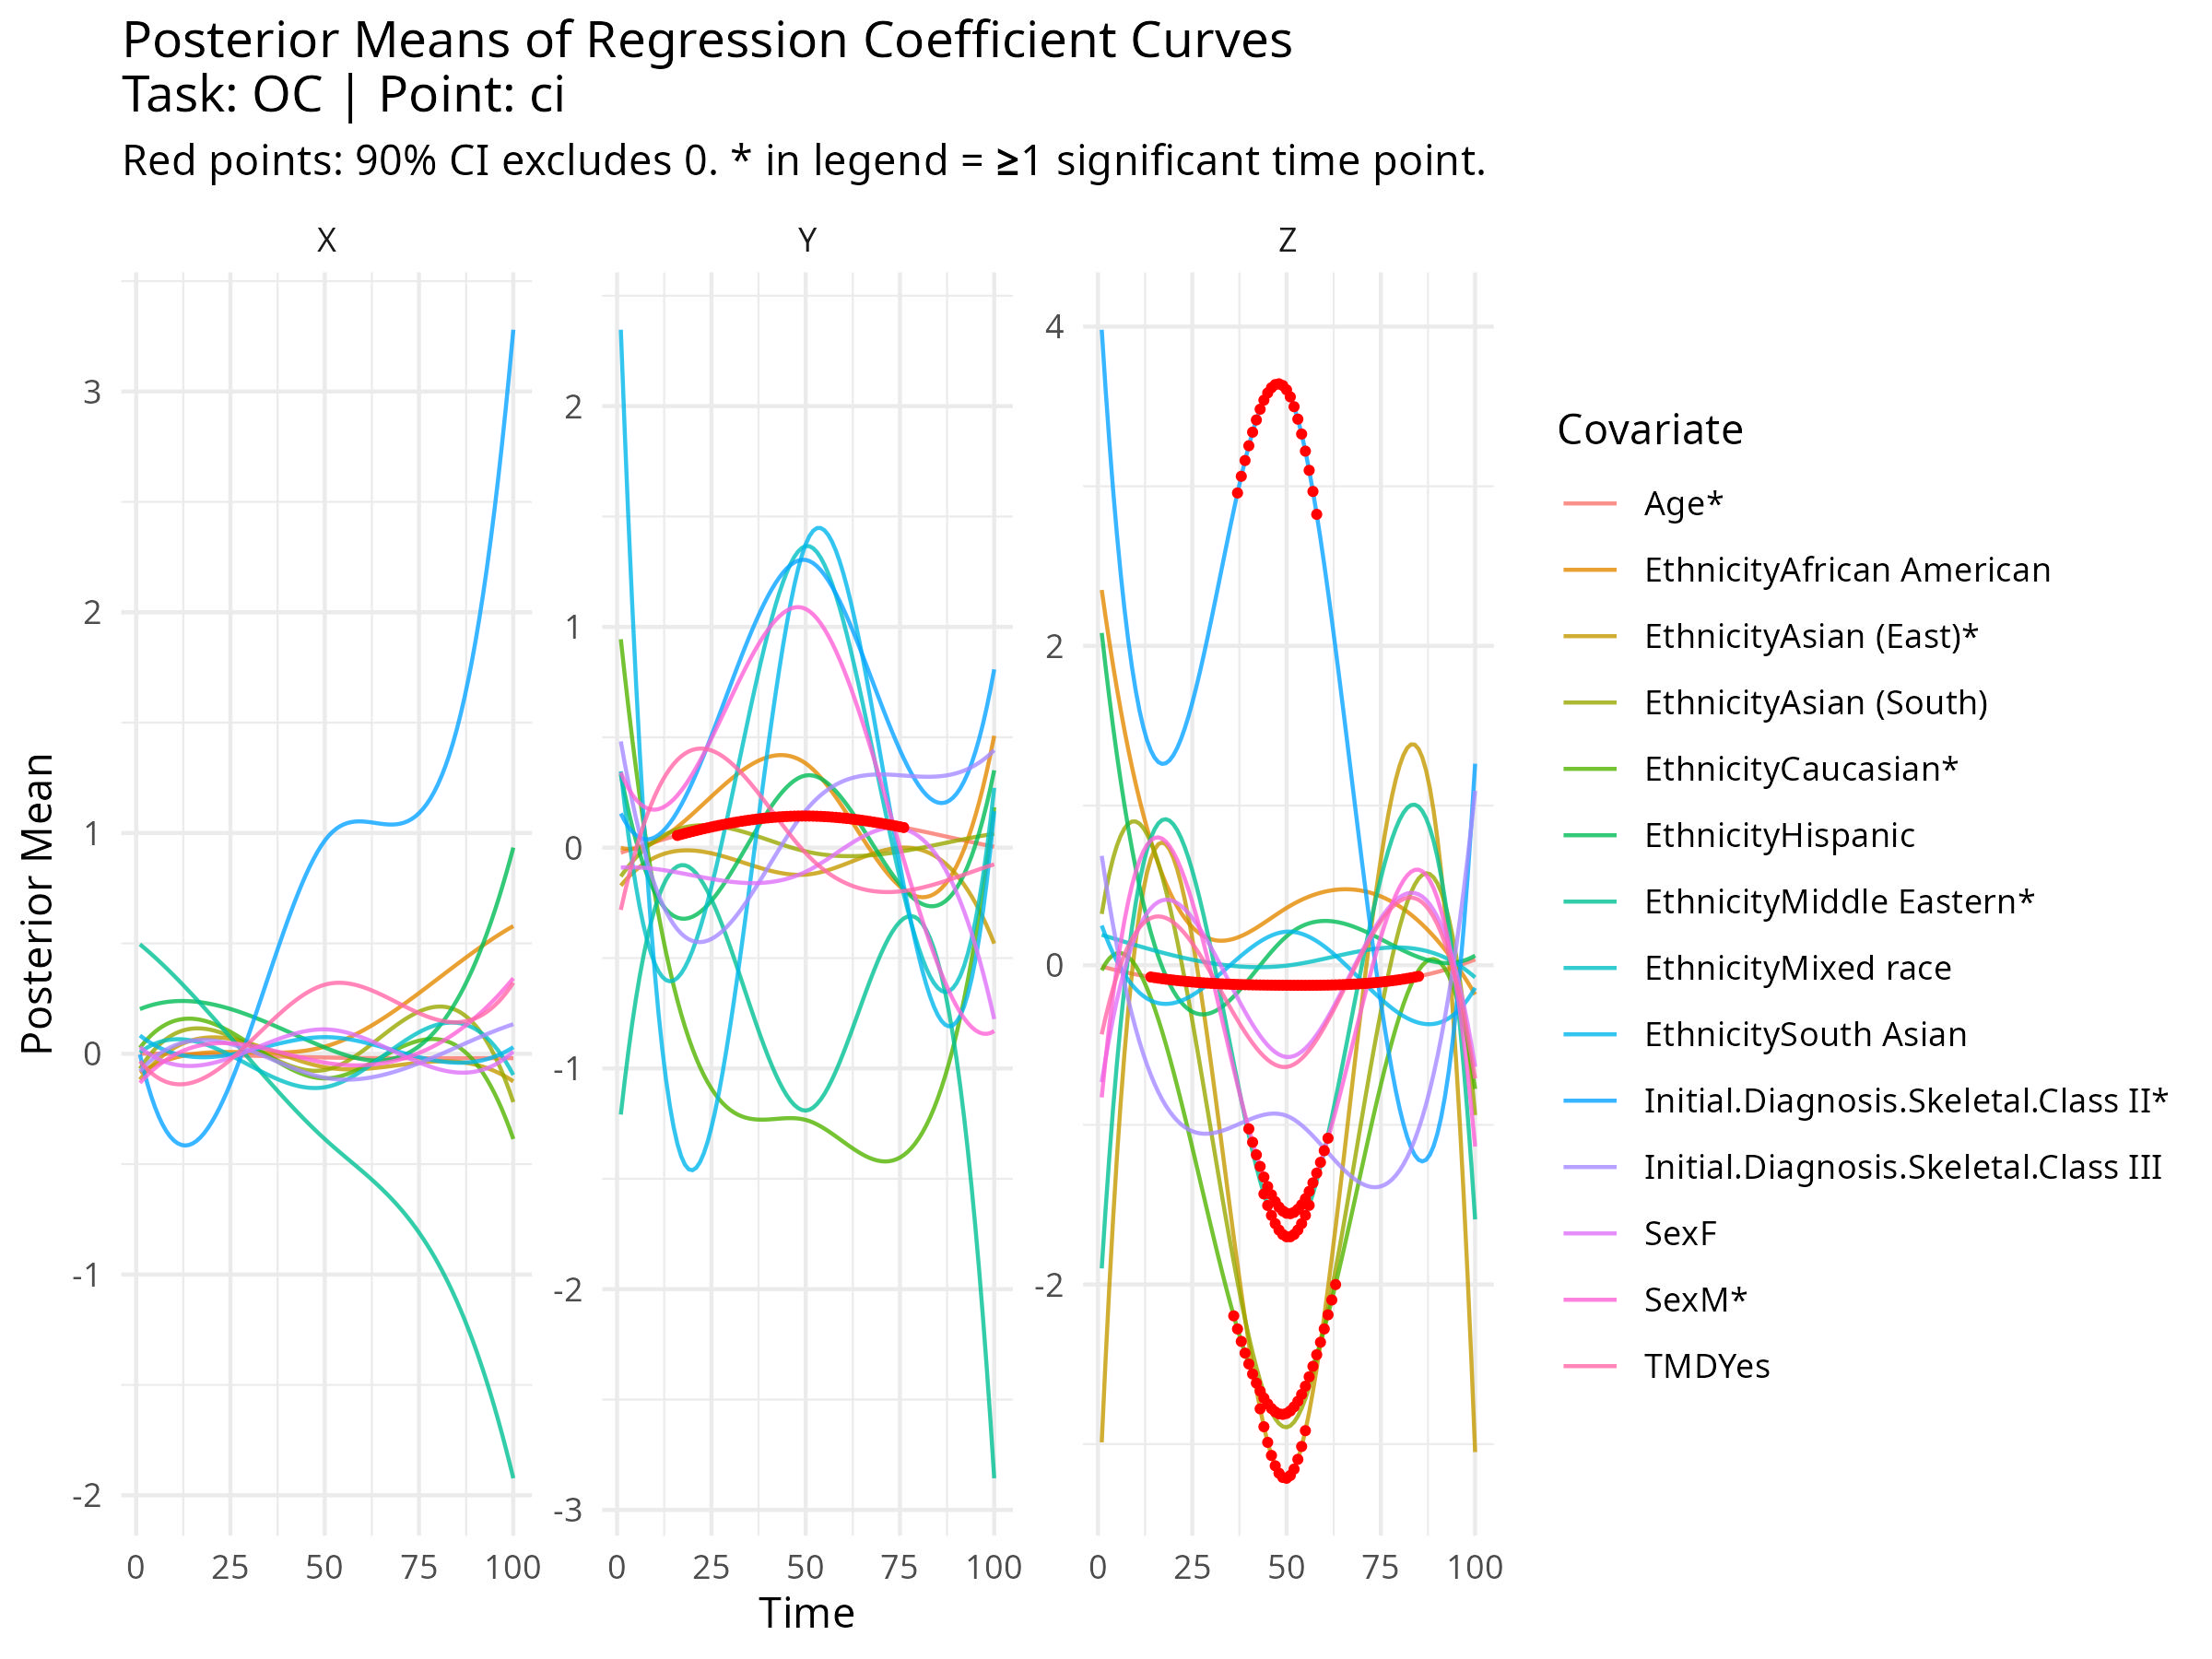
\includegraphics[width = 0.7\textwidth]{oc_ci_plot.jpeg}
    \caption{Results for Open/Close Task, central encisor tracking point.}
    \label{fig:oc_ci}
\end{figure}

\begin{figure}[h]
    \centering
    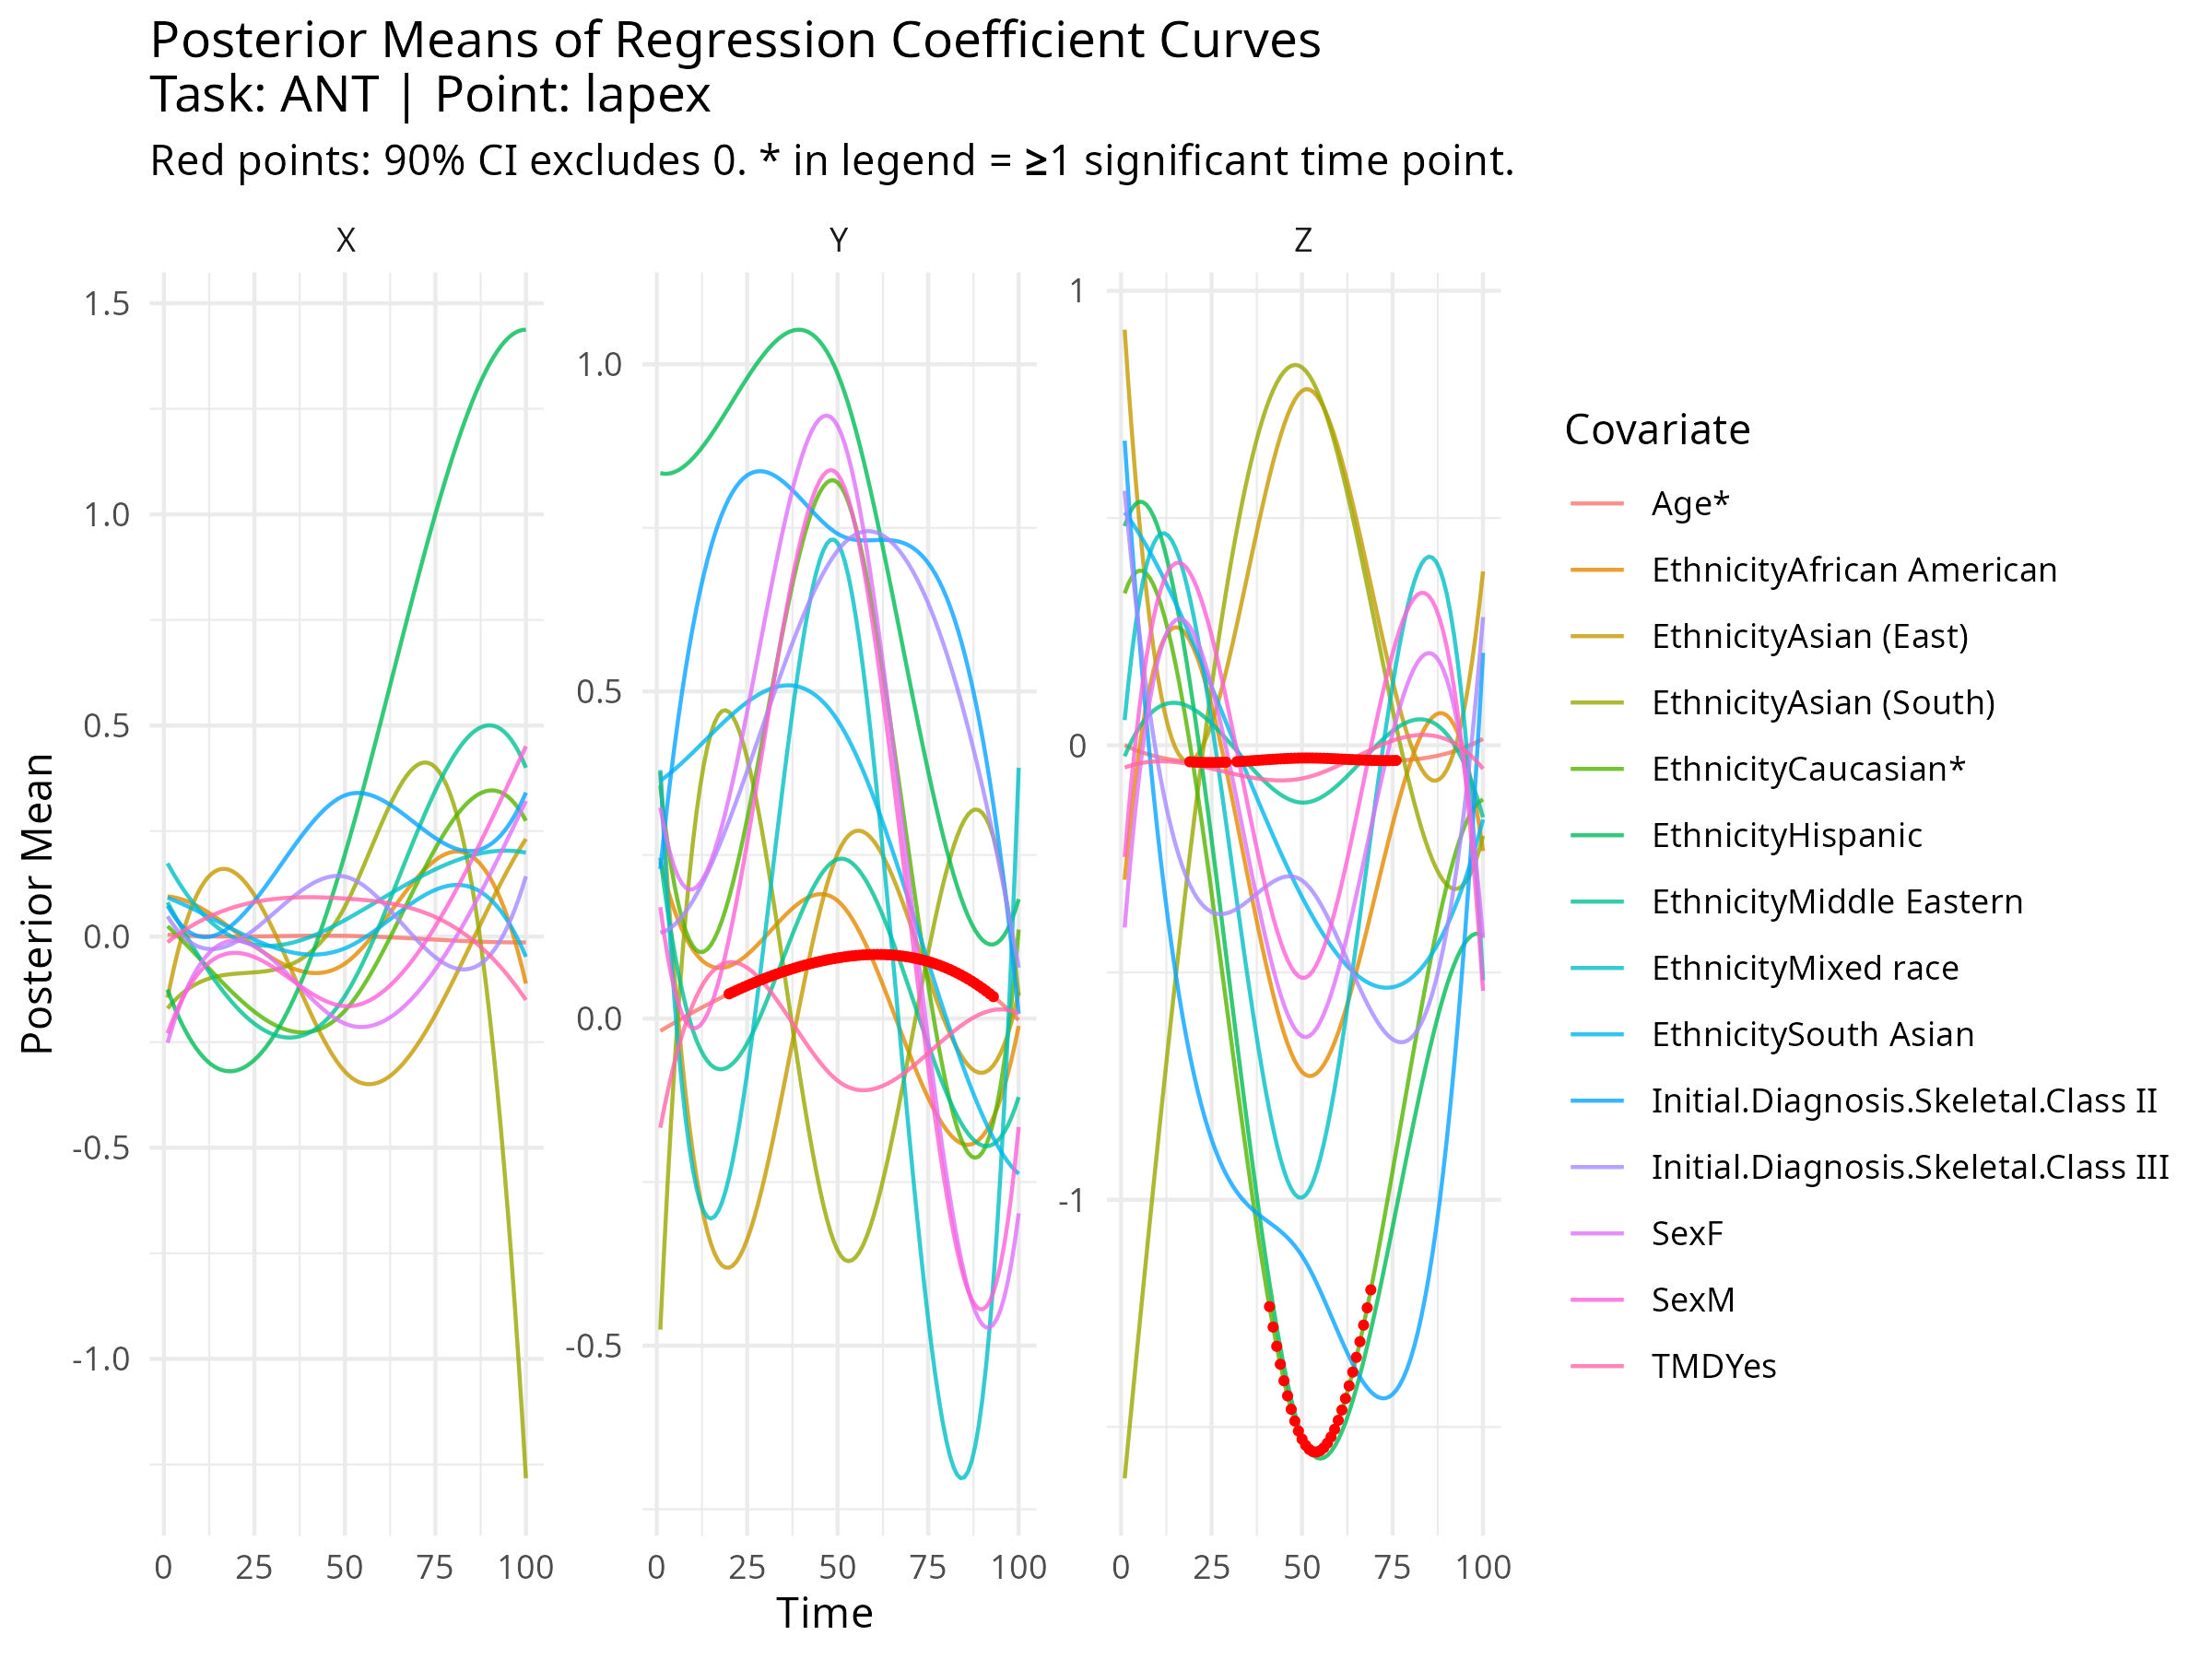
\includegraphics[width = 0.7\textwidth]{ant_lapex_plot.jpeg}
    \caption{Results for Anterior Task, left apex tracking point.}
    \label{fig:ant_lapex}
\end{figure}

A table in the appendix details the significant variables.  The covariate age is the most consistently significant variable; it is significant across all tasks and at all tracking points.  Additionally, it is significant across a wide range of time points.  Sex is another covariate that is very commonly significant, though typically over shorter windows of time than age.  Various ethnicities are also commonly significant, though mostly in the Z dimension and like sex, across shorter time spans than age.  Skeletal class also seems to mostly significant in the Z dimension, likewise at shorter windows of time than age.  The Presence of TMD symptoms is significant only in limited contexts (at one task, one tracking point, and only from time 40 to 62).  

\section{Conclusions}\label{sec5}
The purpose of this work has been to on the using functional regression to analyze three dimensional kinematic data.  Our main model is an extension of an existing method, allowing for the modelling of mean effects, subject level random effects, and correlated errors across all three dimensions.  Attempting to simplify the model estimation by moving a large covariance structure into the random and fixed effects did not work as well as was hoped.  

Despite this, analysis was performed using a modified version of an existing Gibbs sampler, , which provided stable estimation while retaining flexibility in the modeling framework. This approach allowed us to identify covariates that exert consistent and interpretable effects on jaw motion.  In particular, age emerged as the most robust and persistent factor, while sex, ethnicity, and skeletal class were significant in more localized contexts, typically in the Z dimension and over shorter time spans. The presence of TMD symptoms was found to have only limited impact, significant in a restricted set of tasks, points, and time intervals.

More generally, this work demonstrates that high-dimensional functional outcomes, when  carefully structured, via hierarchical models for example, can yield interpretable insights while maintaining statistical rigor.

There are numerous avenues for future exploration of this work's results.  One such idea could be the inclusion of the selection of the roughness penalty \(\alpha\) into the model instead of selecting it \emph{a priori}.  This would make the model truly Bayesian, in the sense that the data would select the smoothness penalty.  

%\backmatter
\bmsection*{Author contributions}

This is an author contribution text. This is an author contribution text. This is an author contribution text. This is an author contribution text. This is an author contribution text.

\bmsection*{Acknowledgments}
We gratefully acknowledge use of TMJ kinematics data obtained through NIH grant U01DE031512 (H. Yao and J. Lee, PIs). 


\bmsection*{Financial disclosure}

None reported.

\bmsection*{Conflict of interest}

The authors declare no potential conflict of interests.

%\bibliography{wileyNJD-AMA}
%\bibliographystyle{wileyNJD-AMA}
\bibliography{references}

\bmsection*{Supporting information}

Additional supporting information may be found in the
online version of the article at the publisher’s website.


\appendix

\bmsection{Tables\label{app1}}

%need to insert the real table here 
\begin{table}[h]
\centering
\begin{tabular}{l|l}
\hline
  & Overall\\
\hline
Number of Patients & 40\\
\hline
\hline
Sex (\%) & \\
\hline
M & 15 (37.5)\\
F & 25(62.5) \\
\hline
\hline
Age (mean (SD)) & 32.73 (14.81)\\
\hline
\hline
Ethnicity (\%) & \\
\hline
African & 1 (2.5)\\
African American & 12 (30.0)\\
Asian (East) & 1 (2.5)\\
Asian (South) & 1 (2.5)\\
Caucasian & 18 (45.0)\\
Hispanic & 1 (2.5)\\
Middle Eastern & 1 (2.5)\\
Mixed race & 3 (7.5)\\
South Asian & 2 (5.0)\\
\hline
\hline
Initial.Diagnosis.Skeletal. (\%) & \\
\hline
Class I & 12 (30.0)\\
Class II & 6 (15.0)\\
Class III & 22 (55.0)\\
\hline
\hline
TMD (\%)  & \\
\hline
Yes & 16 (40.0)\\
No  & 24 (60.0)\\
\hline
\hline
\end{tabular}
\caption{Summary of Covariates}
    \label{tab:description}
\end{table}

\begin{sidewaystable}[h]
    \centering
    % Uncomment the next two lines if your table is too wide:
    % \begin{adjustbox}{max width=\textwidth}
\begin{tabular}{rrrrrrrrrrrrr}
\toprule
D &  Kt\_gen &  Kt\_sample &  p &  I &  var\_fixed &  var\_random &  mean.stan.coverages &  imse.stan &  mean.gibbs.coverages &  imse.gibbs &  stan\_times &  gibbs\_times \\
\midrule
25 &       5 &          5 &  3 & 50 &     0.1000 &      0.1000 &               0.9040 &     0.0598 &                1.0000 &      0.0608 &    259.1143 &    3240.8970 \\
25 &       5 &         10 &  3 & 50 &     0.1000 &      0.1000 &               0.9907 &     0.0638 &                1.0000 &      0.0607 &   1833.2448 &    7025.7435 \\
25 &       5 &          5 & 10 & 50 &     0.1000 &      0.1000 &               0.8164 &     0.1386 &                0.9100 &      0.1262 &    299.9174 &    4234.6802 \\
25 &       5 &         10 & 10 & 50 &     0.1000 &      0.1000 &               0.9808 &     0.0319 &                0.9997 &      0.0289 &   1113.6958 &   14491.6006 \\
25 &       5 &          5 &  3 & 50 &     1.0000 &      0.1000 &               0.9280 &     0.0064 &                1.0000 &      0.0067 &    262.2866 &    3242.2934 \\
25 &       5 &         10 &  3 & 50 &     1.0000 &      0.1000 &               0.9693 &     0.0069 &                1.0000 &      0.0070 &    915.1414 &    7037.9875 \\
25 &       5 &          5 & 10 & 50 &     1.0000 &      0.1000 &               0.7984 &     0.0162 &                0.8704 &      0.0172 &    306.5938 &    4235.3996 \\
25 &       5 &         10 & 10 & 50 &     1.0000 &      0.1000 &               0.9796 &     0.0039 &                0.9995 &      0.0039 &   1179.2835 &   14479.8795 \\
25 &       5 &          5 &  3 & 50 &     0.1000 &      1.0000 &               0.9960 &     0.1054 &                1.0000 &      0.1036 &    277.2761 &    3224.6706 \\
25 &       5 &         10 &  3 & 50 &     0.1000 &      1.0000 &               1.0000 &     0.1268 &                1.0000 &      0.1224 &    638.9297 &    7026.6621 \\
25 &       5 &          5 & 10 & 50 &     0.1000 &      1.0000 &               0.8964 &     0.1487 &                0.9796 &      0.1501 &    316.9695 &    4221.2304 \\
25 &       5 &         10 & 10 & 50 &     0.1000 &      1.0000 &               0.9916 &     0.0715 &                1.0000 &      0.0940 &    838.7632 &   14462.8522 \\
25 &       5 &          5 &  3 & 50 &     1.0000 &      1.0000 &               0.9947 &     0.0116 &                1.0000 &      0.0117 &    280.4149 &    3234.2076 \\
25 &       5 &         10 &  3 & 50 &     1.0000 &      1.0000 &               0.9840 &     0.0161 &                1.0000 &      0.0159 &    786.4246 &    7029.5817 \\
25 &       5 &          5 & 10 & 50 &     1.0000 &      1.0000 &               0.8780 &     0.0178 &                0.9688 &      0.0211 &    318.1880 &    4229.4626 \\
25 &       5 &         10 & 10 & 50 &     1.0000 &      1.0000 &               0.9884 &     0.0099 &                1.0000 &      0.0129 &    862.8026 &   14489.7824 \\
\bottomrule
\end{tabular}

    % \end{adjustbox}
    \caption{Summary of simulation partial results.  Numeric results rounded to four decimal places.}
    \label{tab:simulation_results}
\end{sidewaystable}

\begin{table}
\centering
\resizebox{\linewidth}{!}{
{%
\renewcommand{\arraystretch}{0.1}
\begin{tabular}[t]{lllll}
\toprule
coef & dim & time\_points & task & tracking\_point\\
\midrule
Age & Y & 18-93 & ant & ci\\
Age & Z & 15-84 & ant & ci\\
EthnicityAfrican American & Z & 42-62 & ant & ci\\
EthnicityAsian (South) & Z & 41-59 & ant & ci\\
EthnicityCaucasian & Z & 39-67 & ant & ci\\
\addlinespace
SexF & Z & 46-52 & ant & ci\\
SexM & Y & 41-54 & ant & ci\\
SexM & Z & 50 & ant & ci\\
Age & Y & 20-93 & ant & lapex\\
Age & Z & 19-29, 32-76 & ant & lapex\\
\addlinespace
EthnicityCaucasian & Z & 41-69 & ant & lapex\\
Age & Y & 18-87 & ant & rapex\\
Age & Z & 10-83 & ant & rapex\\
EthnicityAfrican American & Z & 40-62 & ant & rapex\\
EthnicityAsian (South) & Z & 1, 15-21, 39-63, 81-88 & ant & rapex\\
\addlinespace
EthnicityCaucasian & Y & 42-53 & ant & rapex\\
Initial.Diagnosis.Skeletal.Class III & Z & 32-59 & ant & rapex\\
Age & Z & 41-68 & latL & ci\\
EthnicityAsian (East) & Z & 39-64 & latL & ci\\
EthnicityAsian (South) & Z & 41-62 & latL & ci\\
\addlinespace
EthnicityCaucasian & Z & 42-65 & latL & ci\\
Initial.Diagnosis.Skeletal.Class II & Z & 43-59 & latL & ci\\
Initial.Diagnosis.Skeletal.Class III & Z & 43-60 & latL & ci\\
TMDYes & Z & 40-62 & latL & ci\\
Age & Y & 25-74 & latL & lapex\\
\addlinespace
Age & Z & 20-83 & latL & lapex\\
EthnicityAsian (East) & Z & 38-66 & latL & lapex\\
EthnicityAsian (South) & Z & 47-55 & latL & lapex\\
EthnicitySouth Asian & Z & 39-63 & latL & lapex\\
Initial.Diagnosis.Skeletal.Class III & Z & 41-70 & latL & lapex\\
\addlinespace
SexF & Z & 43-55 & latL & lapex\\
Age & X & 20-78 & latL & rapex\\
Age & Z & 23-86 & latL & rapex\\
SexF & X & 30-69 & latL & rapex\\
SexM & X & 32-68 & latL & rapex\\
\addlinespace
Age & Y & 23-92 & latR & ci\\
Age & Z & 20-83 & latR & ci\\
Initial.Diagnosis.Skeletal.Class II & Z & 34-67 & latR & ci\\
SexF & Y & 40-52 & latR & ci\\
SexF & Z & 42-58 & latR & ci\\
\addlinespace
SexM & Z & 46-53 & latR & ci\\
EthnicityAsian (South) & X & 90-100 & latR & lapex\\
Age & X & 14-86 & latR & rapex\\
Age & Z & 17-86 & latR & rapex\\
SexF & X & 37-59 & latR & rapex\\
\addlinespace
SexM & X & 33-65 & latR & rapex\\
Age & Y & 16-76 & oc & ci\\
Age & Z & 14-85 & oc & ci\\
EthnicityAsian (East) & Z & 43-55 & oc & ci\\
EthnicityCaucasian & Z & 36-63 & oc & ci\\
\addlinespace
EthnicityMiddle Eastern & Z & 44-56 & oc & ci\\
Initial.Diagnosis.Skeletal.Class II & Z & 37-58 & oc & ci\\
SexM & Z & 40-61 & oc & ci\\
Age & Y & 18-70 & oc & lapex\\
Age & Z & 25-83 & oc & lapex\\
\addlinespace
EthnicityCaucasian & Z & 36-60 & oc & lapex\\
EthnicityMiddle Eastern & Z & 40-61 & oc & lapex\\
EthnicitySouth Asian & Z & 45-54 & oc & lapex\\
Initial.Diagnosis.Skeletal.Class II & Z & 41-58 & oc & lapex\\
SexM & Z & 38-62 & oc & lapex\\
\addlinespace
Age & Y & 19-61, 96-100 & oc & rapex\\
Age & Z & 1, 14-90 & oc & rapex\\
EthnicityAfrican American & Z & 35-63 & oc & rapex\\
EthnicityCaucasian & Z & 38-63 & oc & rapex\\
EthnicityHispanic & Z & 46-52 & oc & rapex\\
\addlinespace
EthnicityMiddle Eastern & Z & 43-58 & oc & rapex\\
EthnicityMixed race & Z & 49-55 & oc & rapex\\
Initial.Diagnosis.Skeletal.Class III & Z & 19-79 & oc & rapex\\
SexF & Y & 49-51, 92-100 & oc & rapex\\
SexF & Z & 50-56 & oc & rapex\\
\addlinespace
SexM & Y & 95-100 & oc & rapex\\
SexM & Z & 32-66 & oc & rapex\\
\bottomrule
\end{tabular}}
}%
\caption{Summary of Significant covariates by dimension, time points, task, and tracking point.}
\label{tab:significant_covariates}
\end{table}

\bmsection{Emperical Results\label{app2}}%
\vspace*{12pt}
Below are some more images from the emperical results:

\begin{figure}[h]
    \centering
    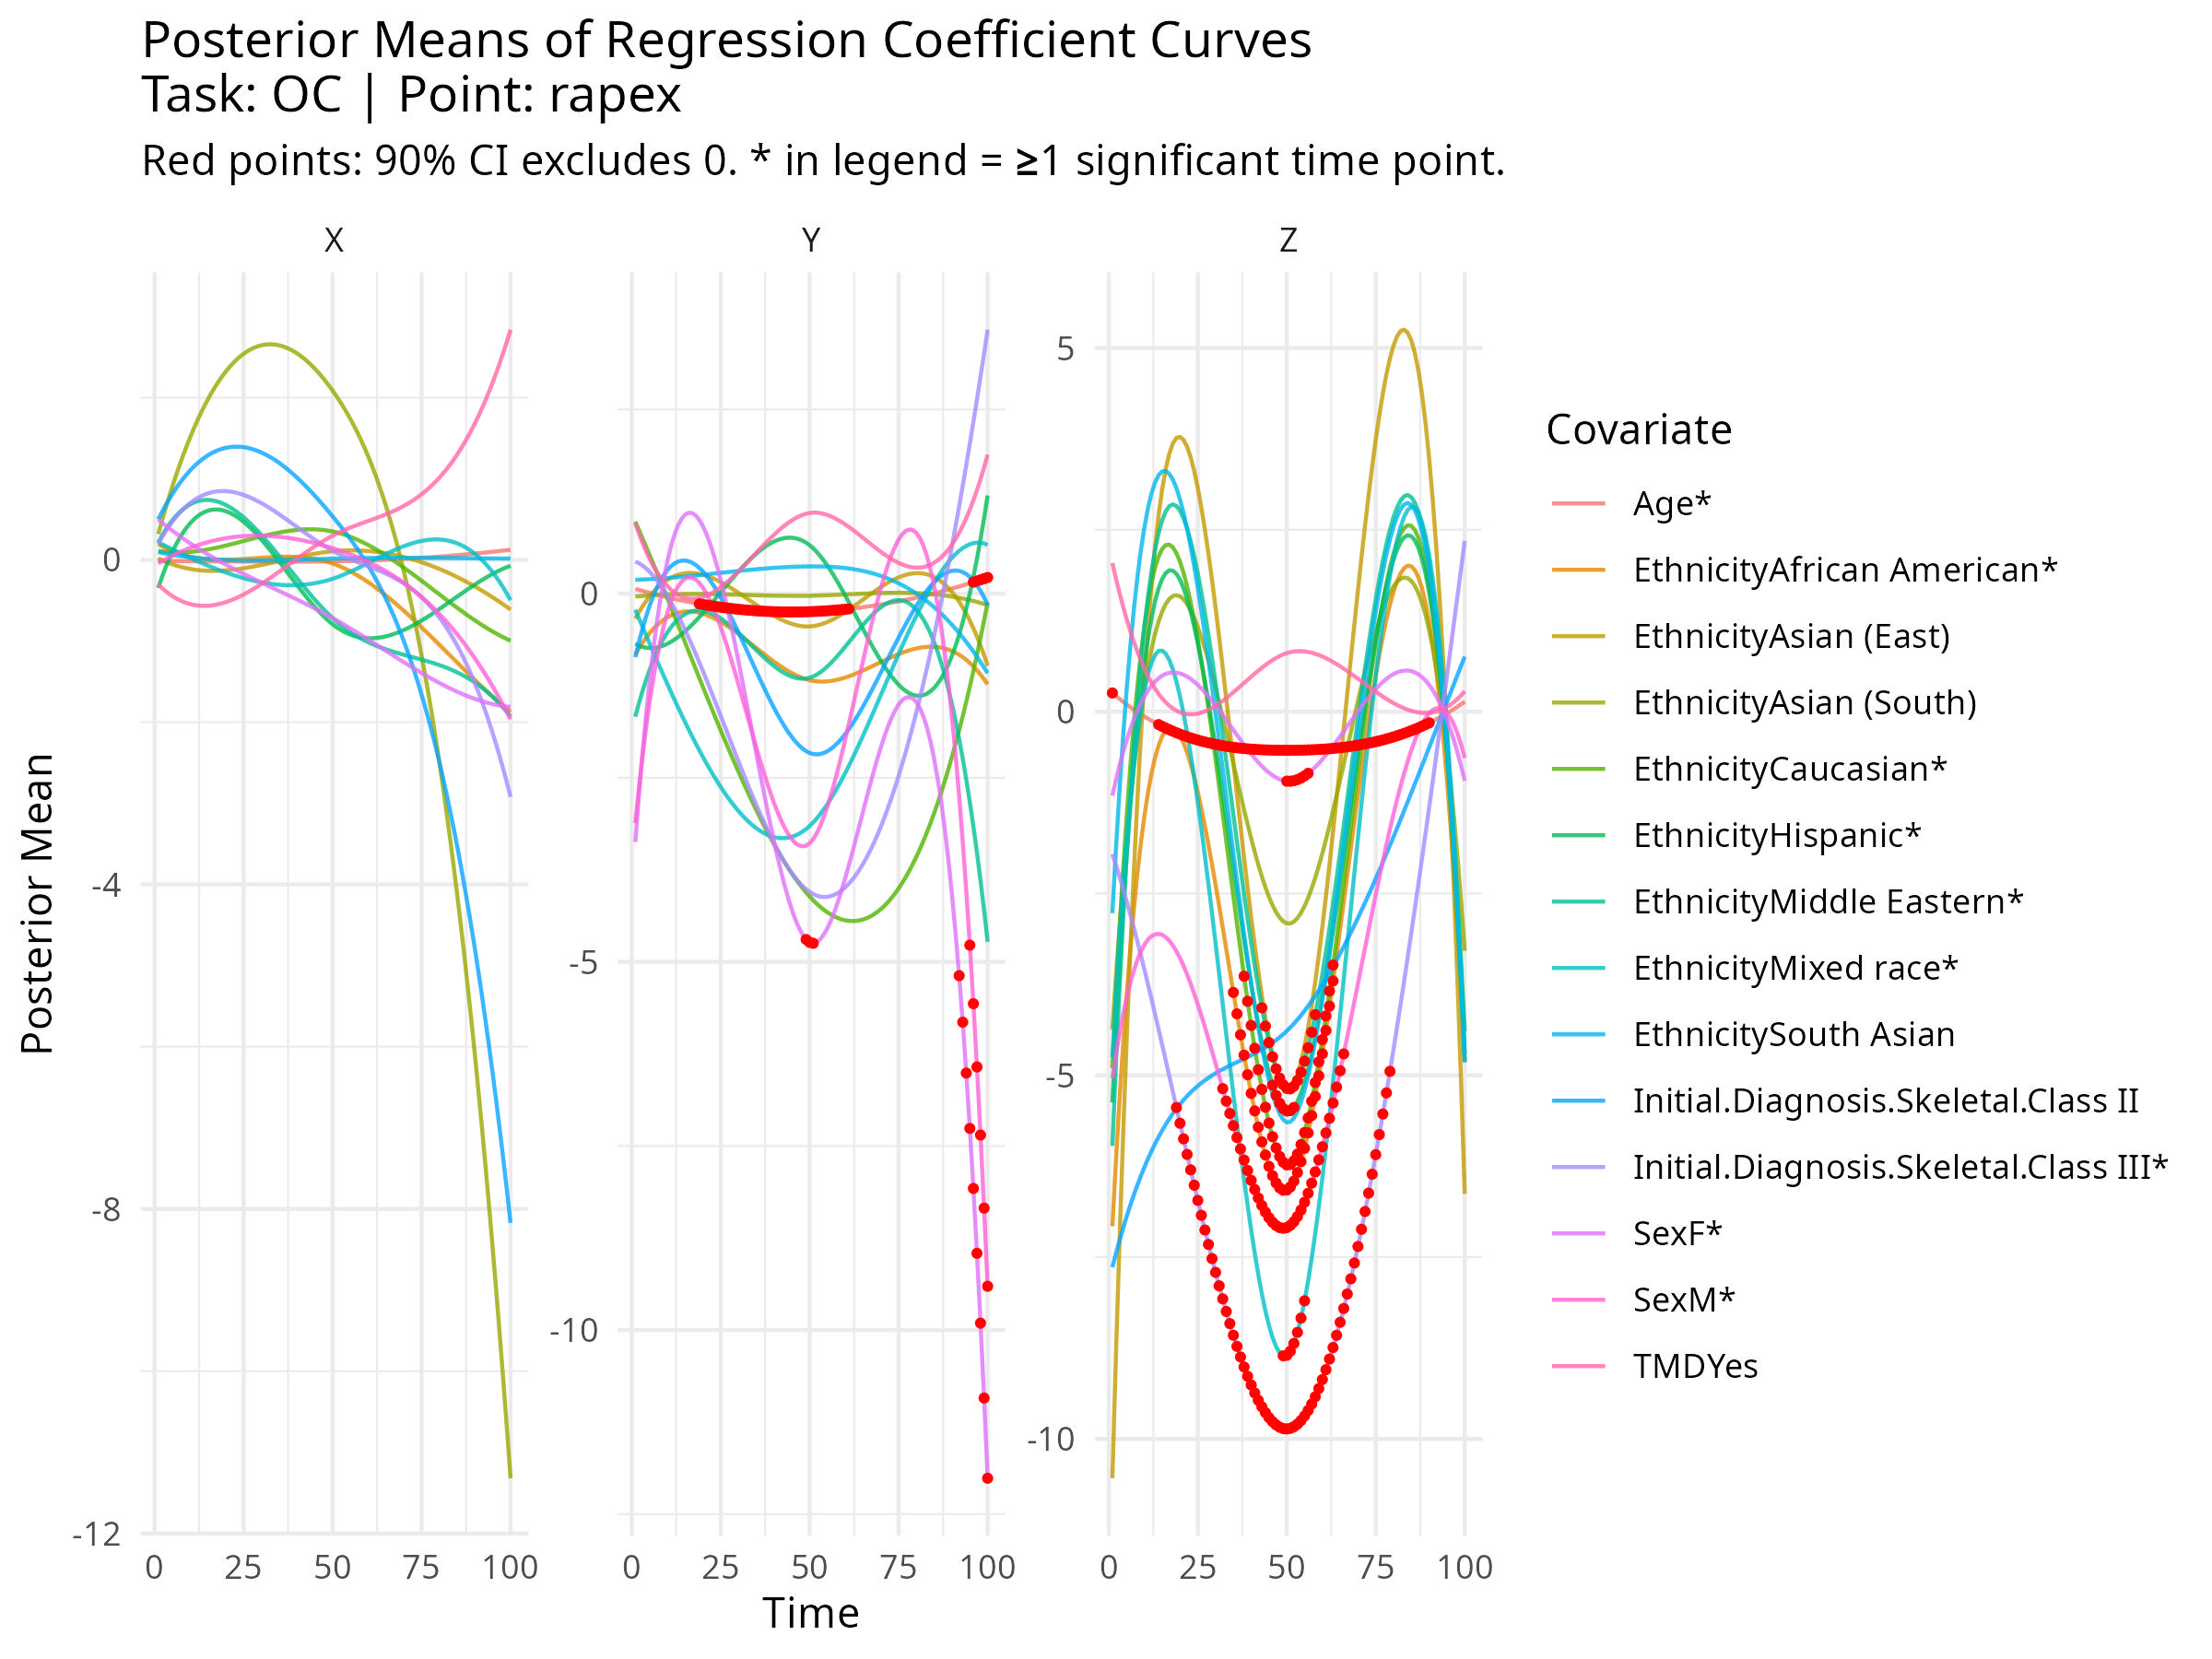
\includegraphics[width = 0.7\textwidth]{oc_rapex_plot.jpeg}
    \caption{Results for Open/Close Task, Right Apex tracking point.}
    \label{fig:oc_rapex}
\end{figure}

\begin{figure}[h]
    \centering
    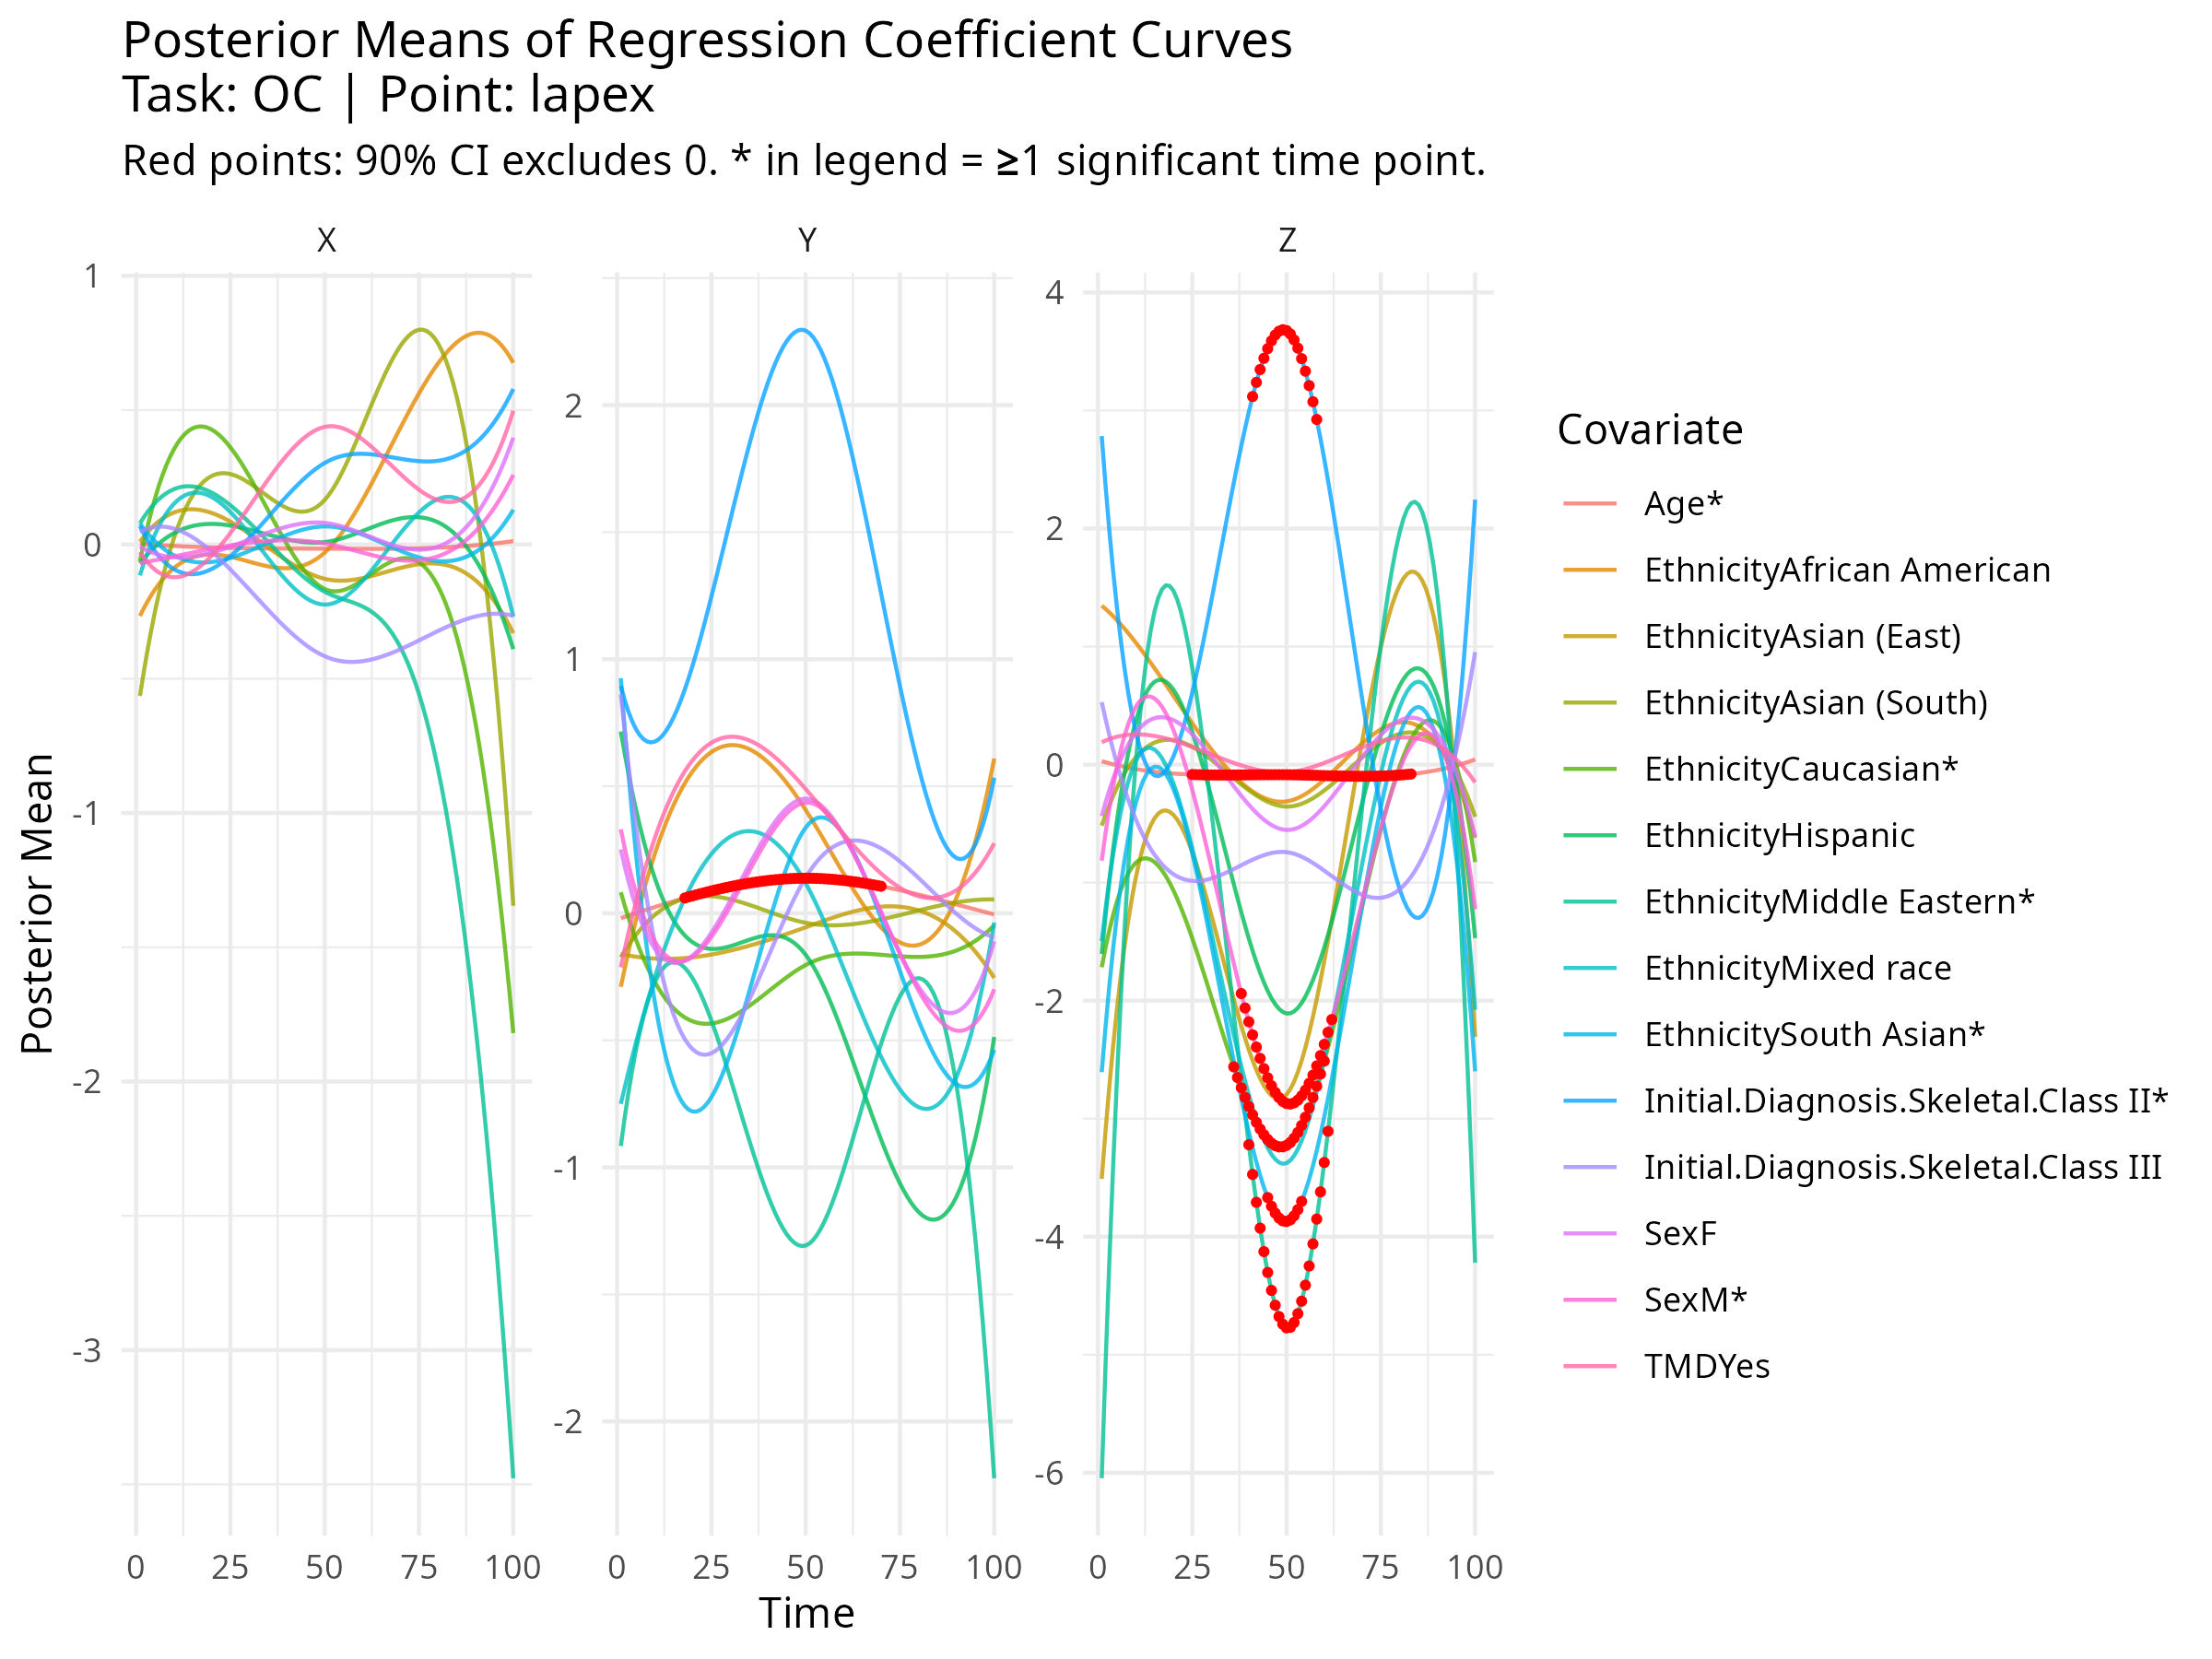
\includegraphics[width = 0.7\textwidth]{oc_lapex_plot.jpeg}
    \caption{Results for Open/Close Task, Left Apex tracking point.}
    \label{fig:oc_lapex}
\end{figure}

\begin{figure}[h]
    \centering
    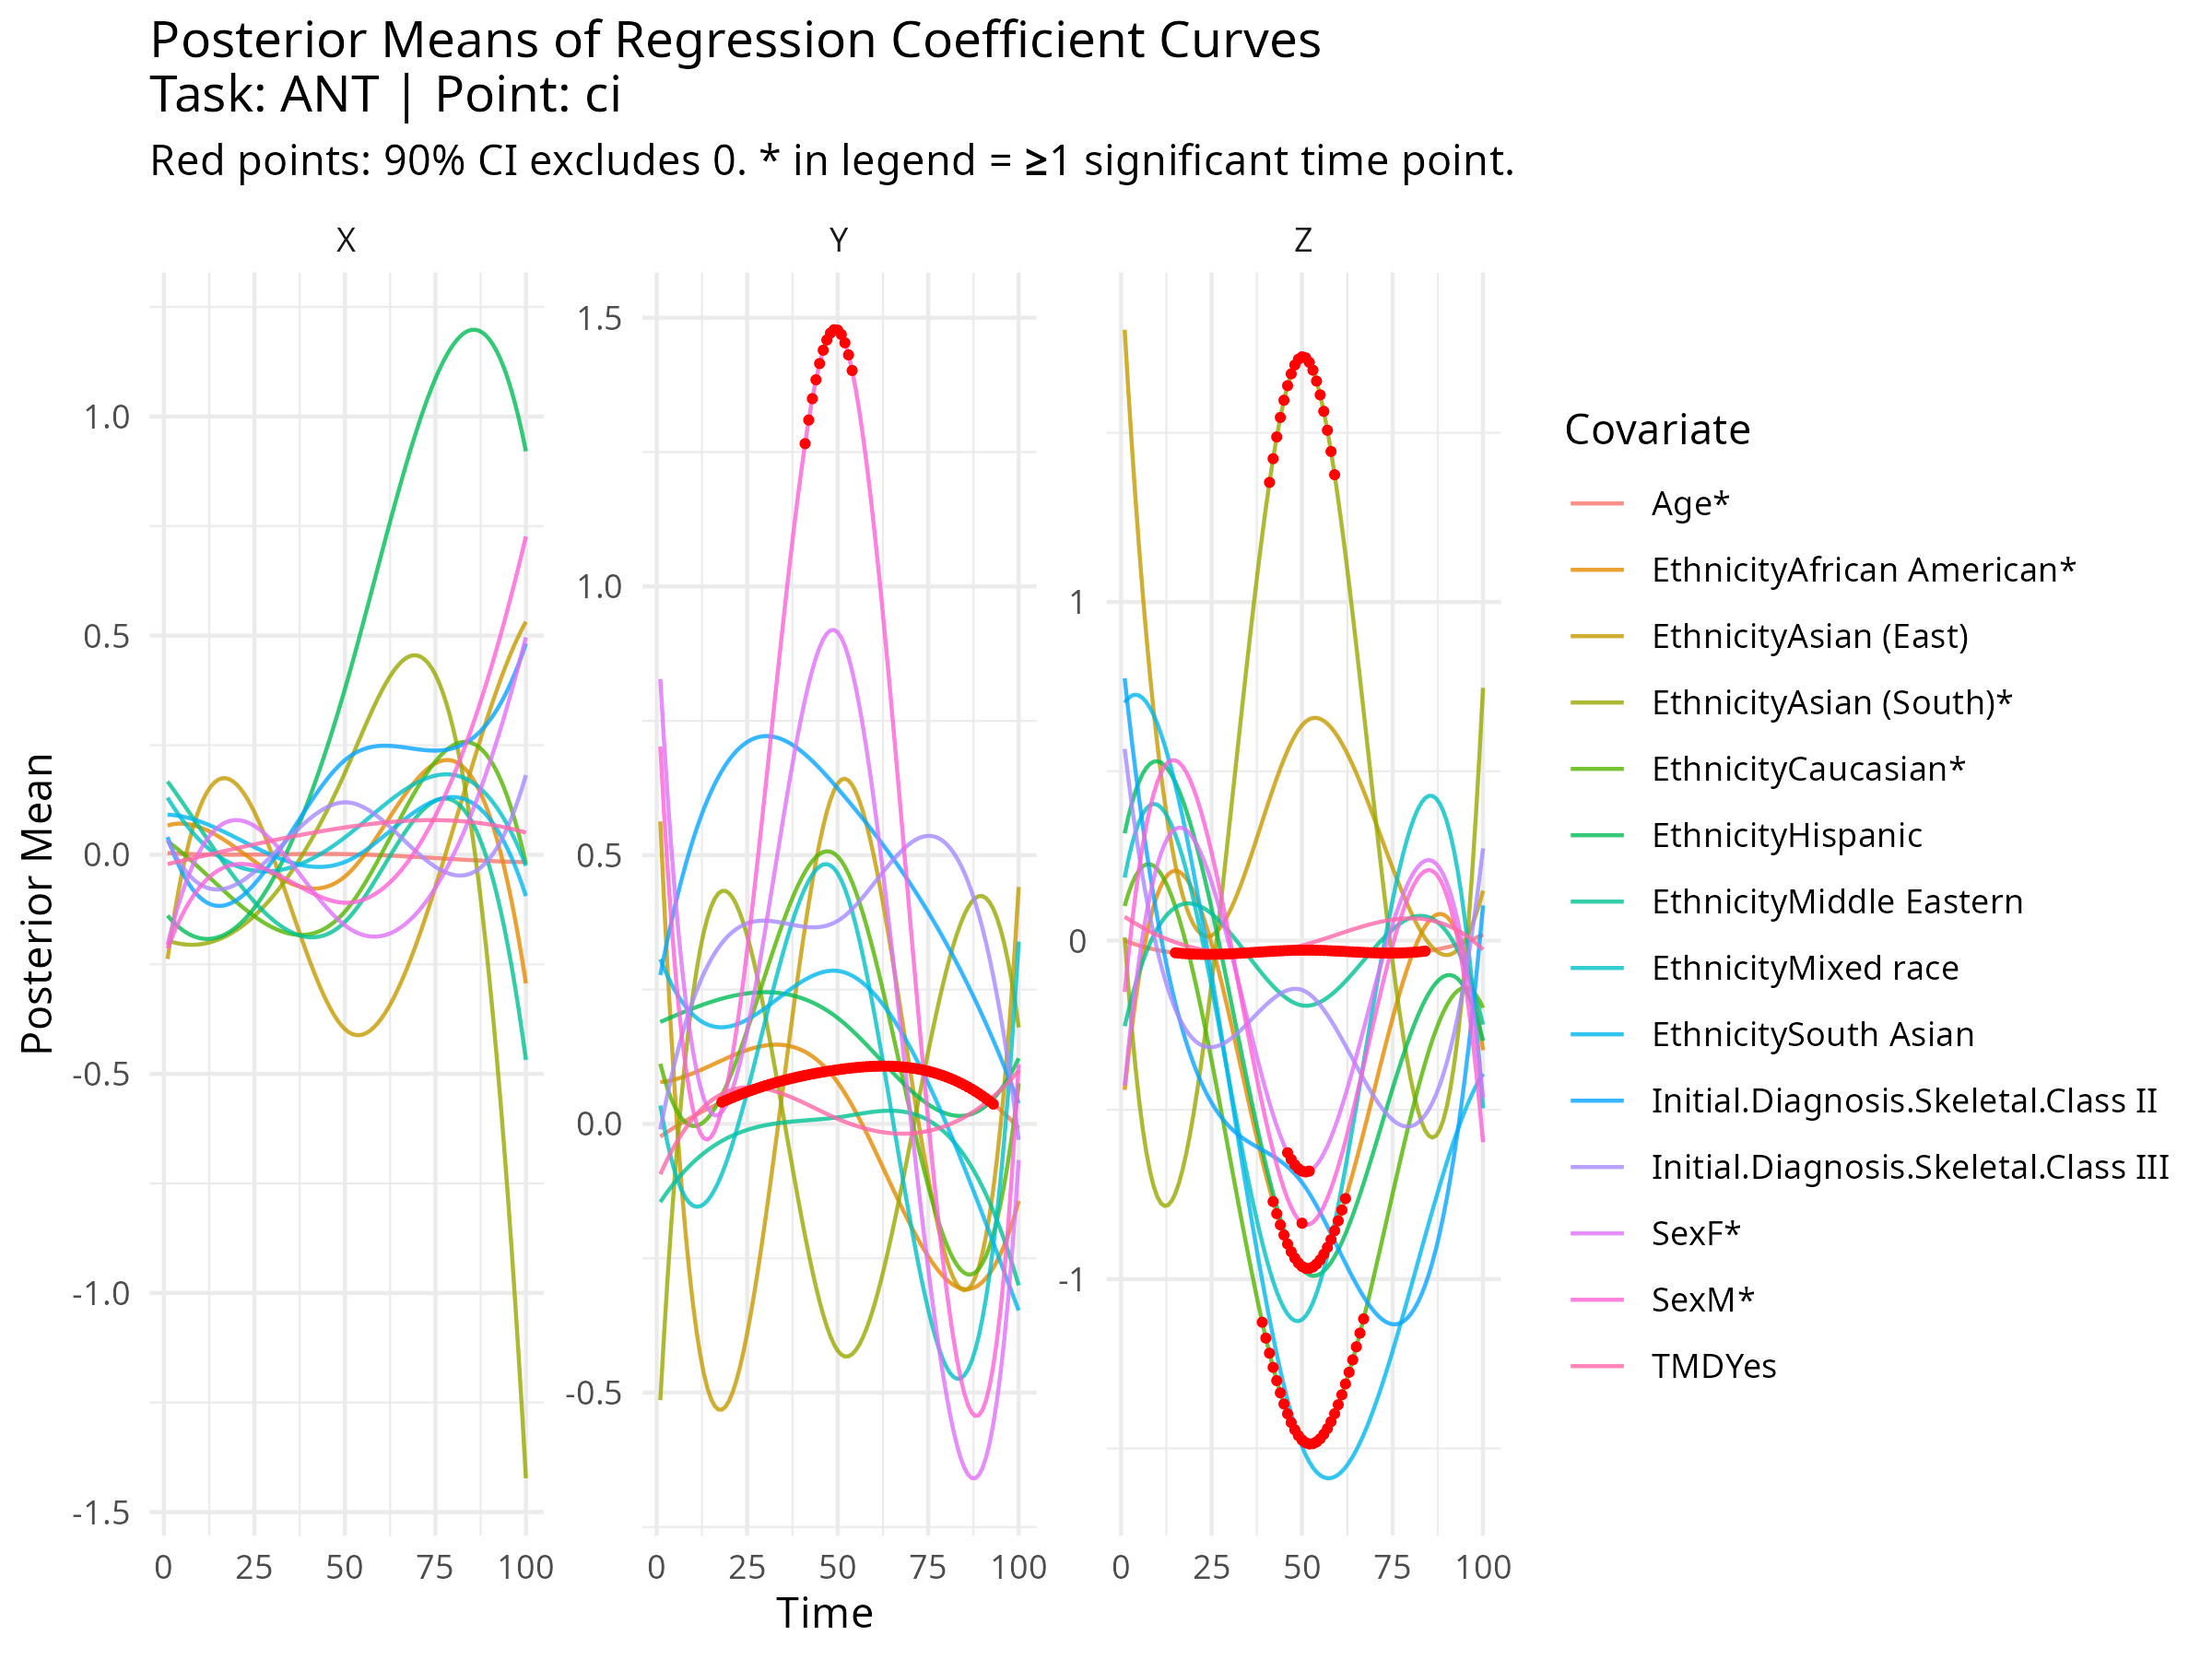
\includegraphics[width = 0.7\textwidth]{ant_ci_plot.jpeg}
    \caption{Results for Anterior Task, Central Incisor tracking point.}
    \label{fig:ant_ci}
\end{figure}

\begin{figure}[h]
    \centering
    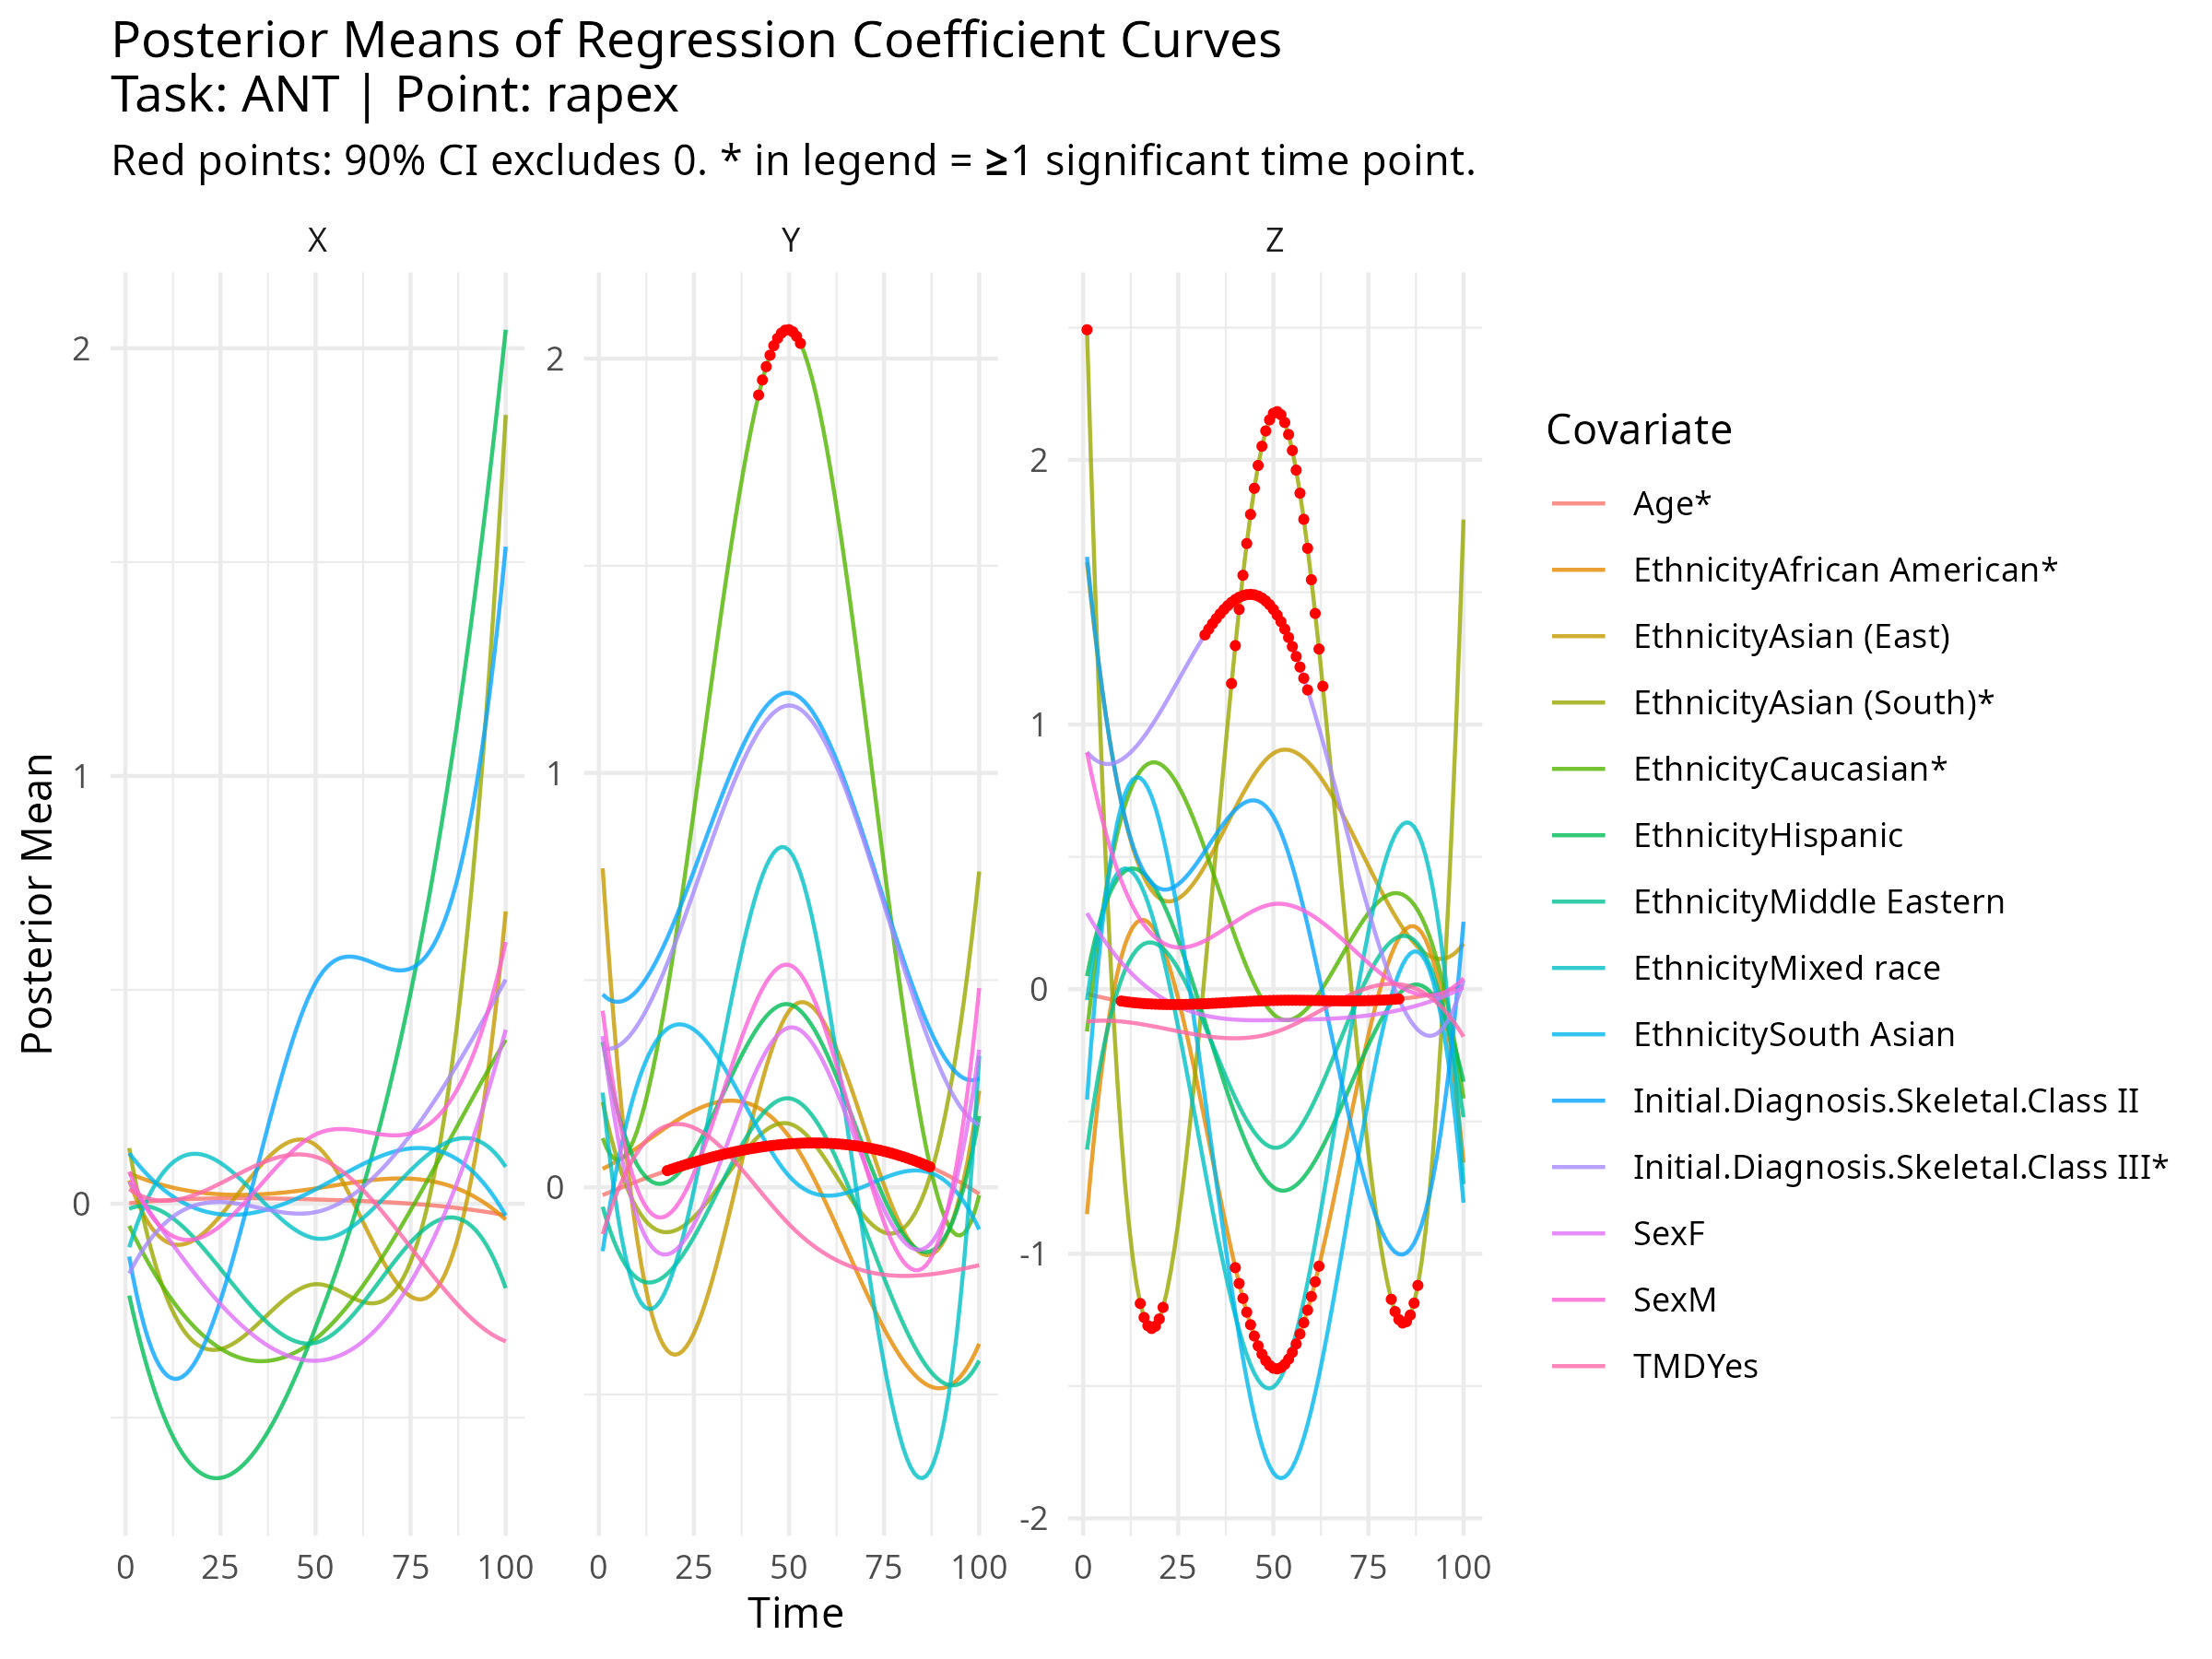
\includegraphics[width = 0.7\textwidth]{ant_rapex_plot.jpeg}
    \caption{Results for Anterior Task, Right Apex tracking point.}
    \label{fig:ant_rapex}
\end{figure}

\begin{figure}[h]
    \centering
    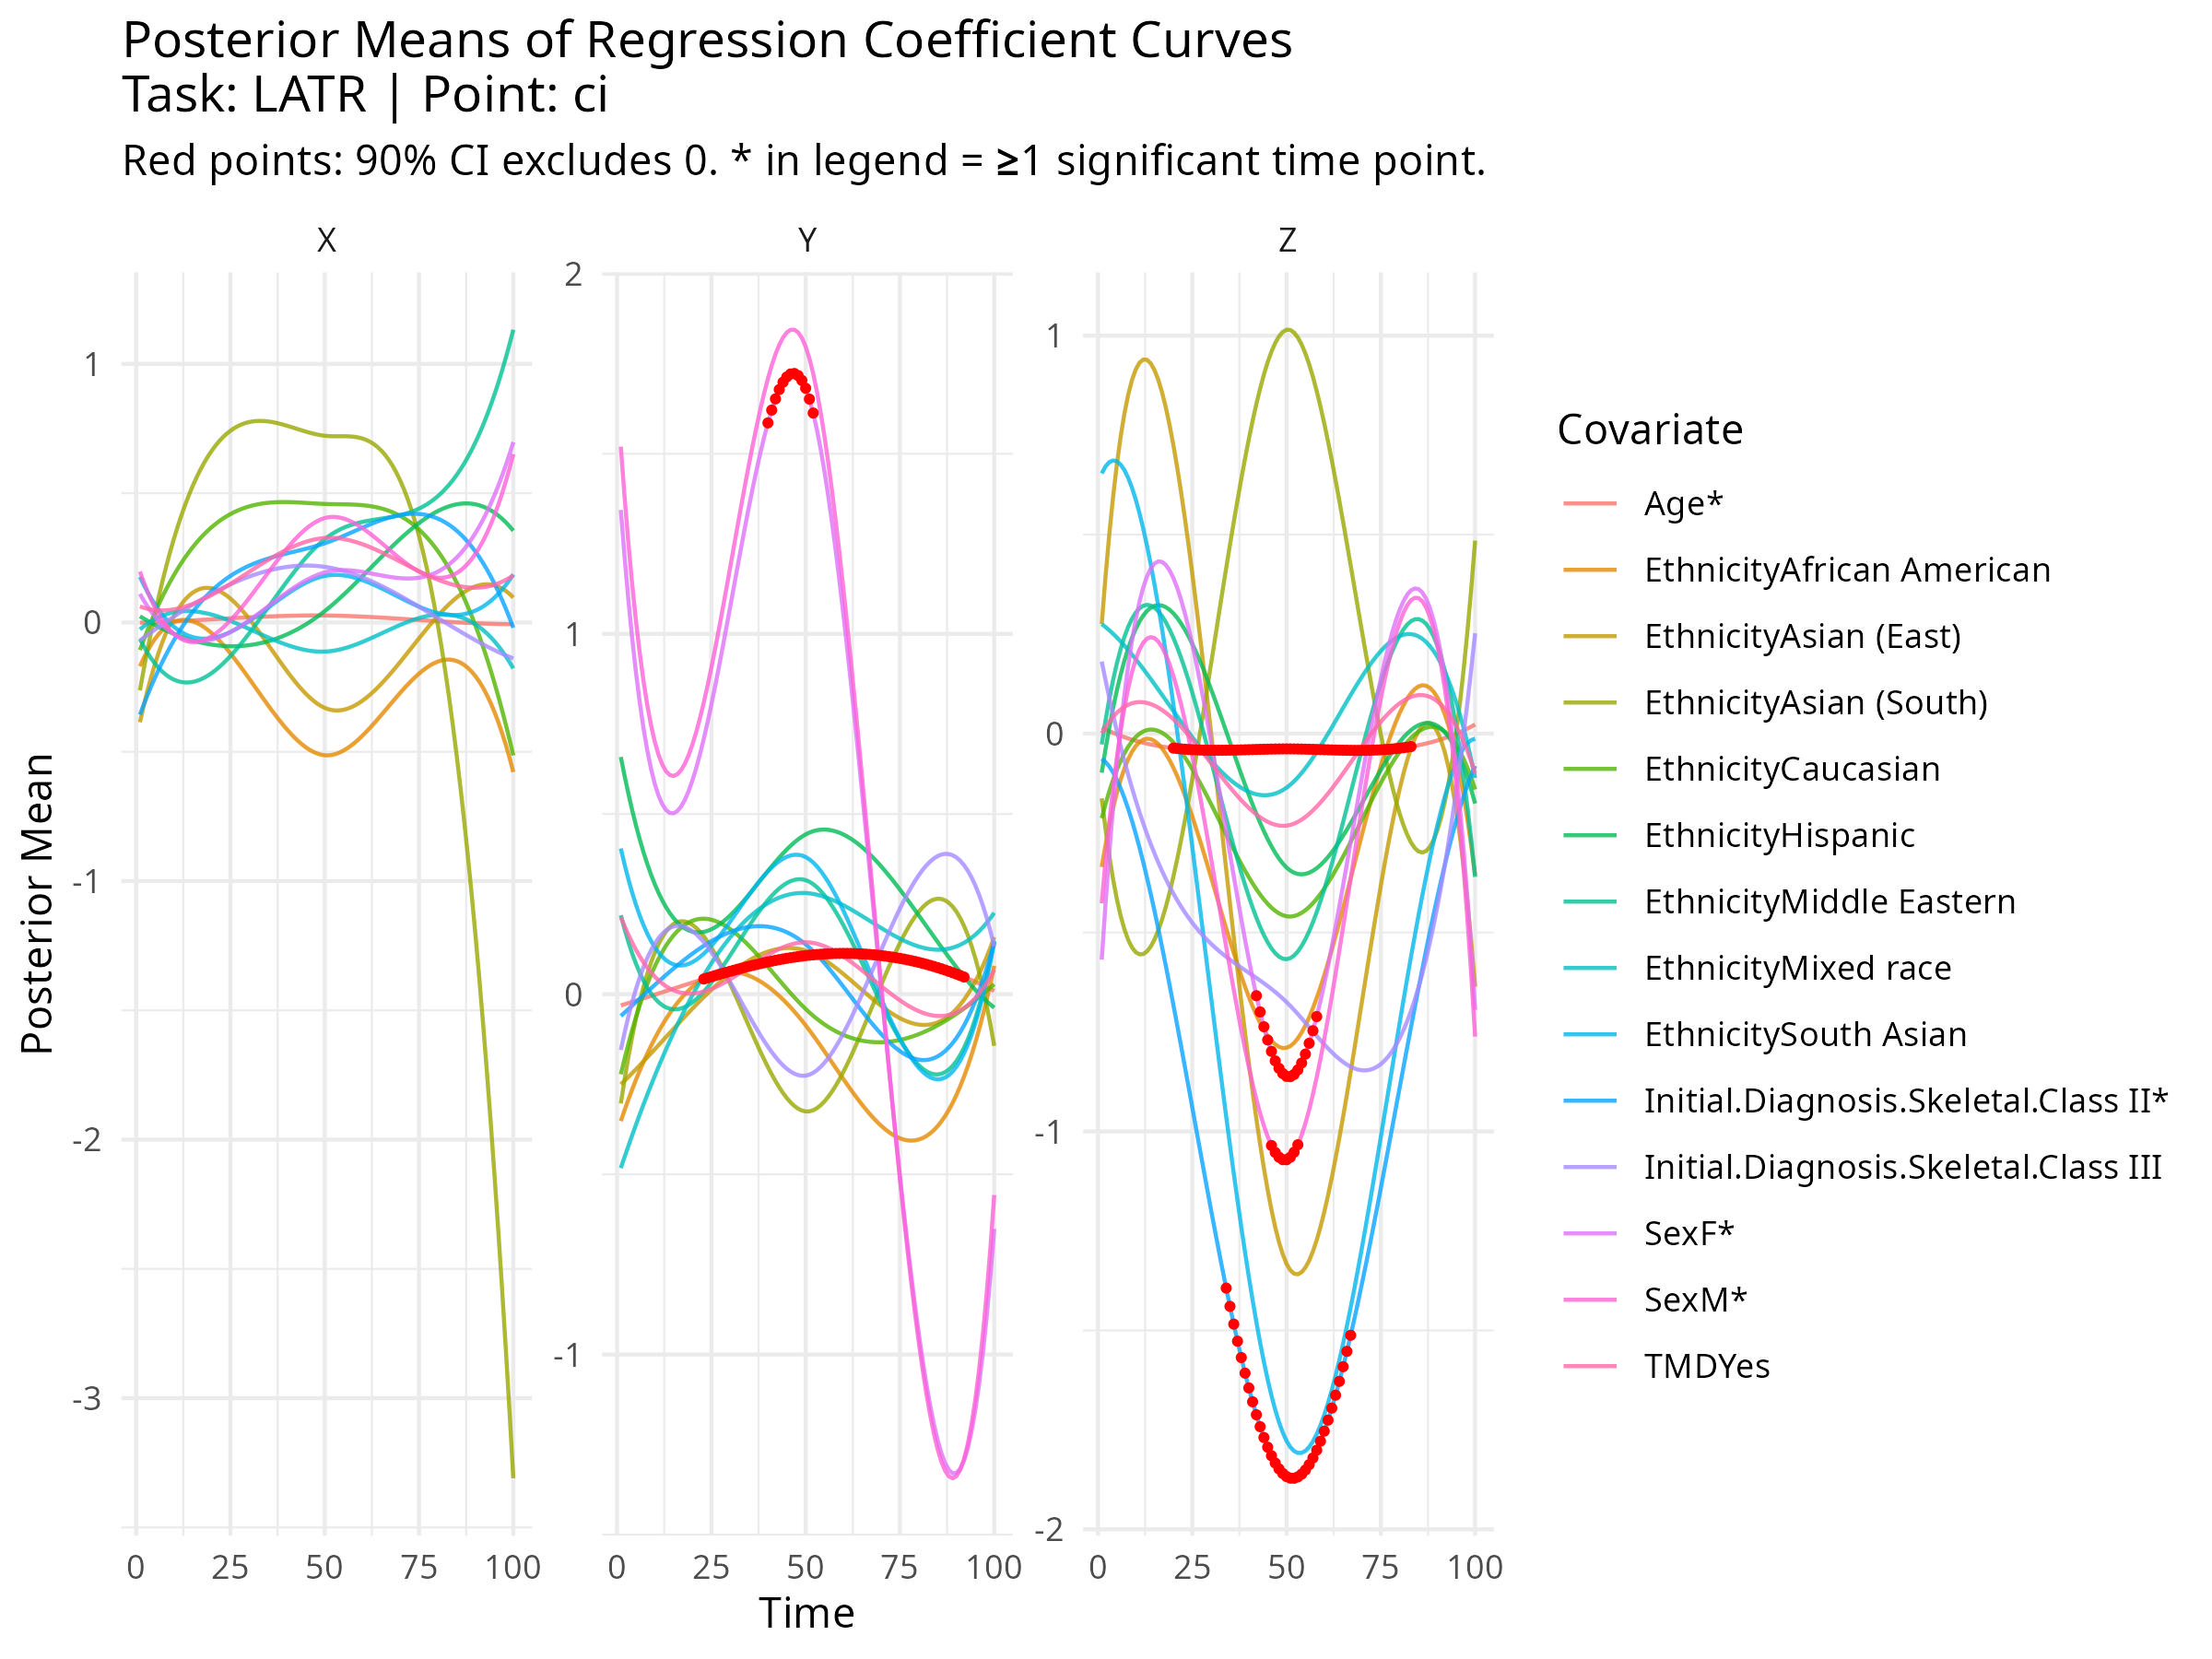
\includegraphics[width = 0.7\textwidth]{latR_ci_plot.jpeg}
    \caption{Results for Lateral Right Task, Central Incisor tracking point.}
    \label{fig:latR_ci}
\end{figure}

\begin{figure}[h]
    \centering
    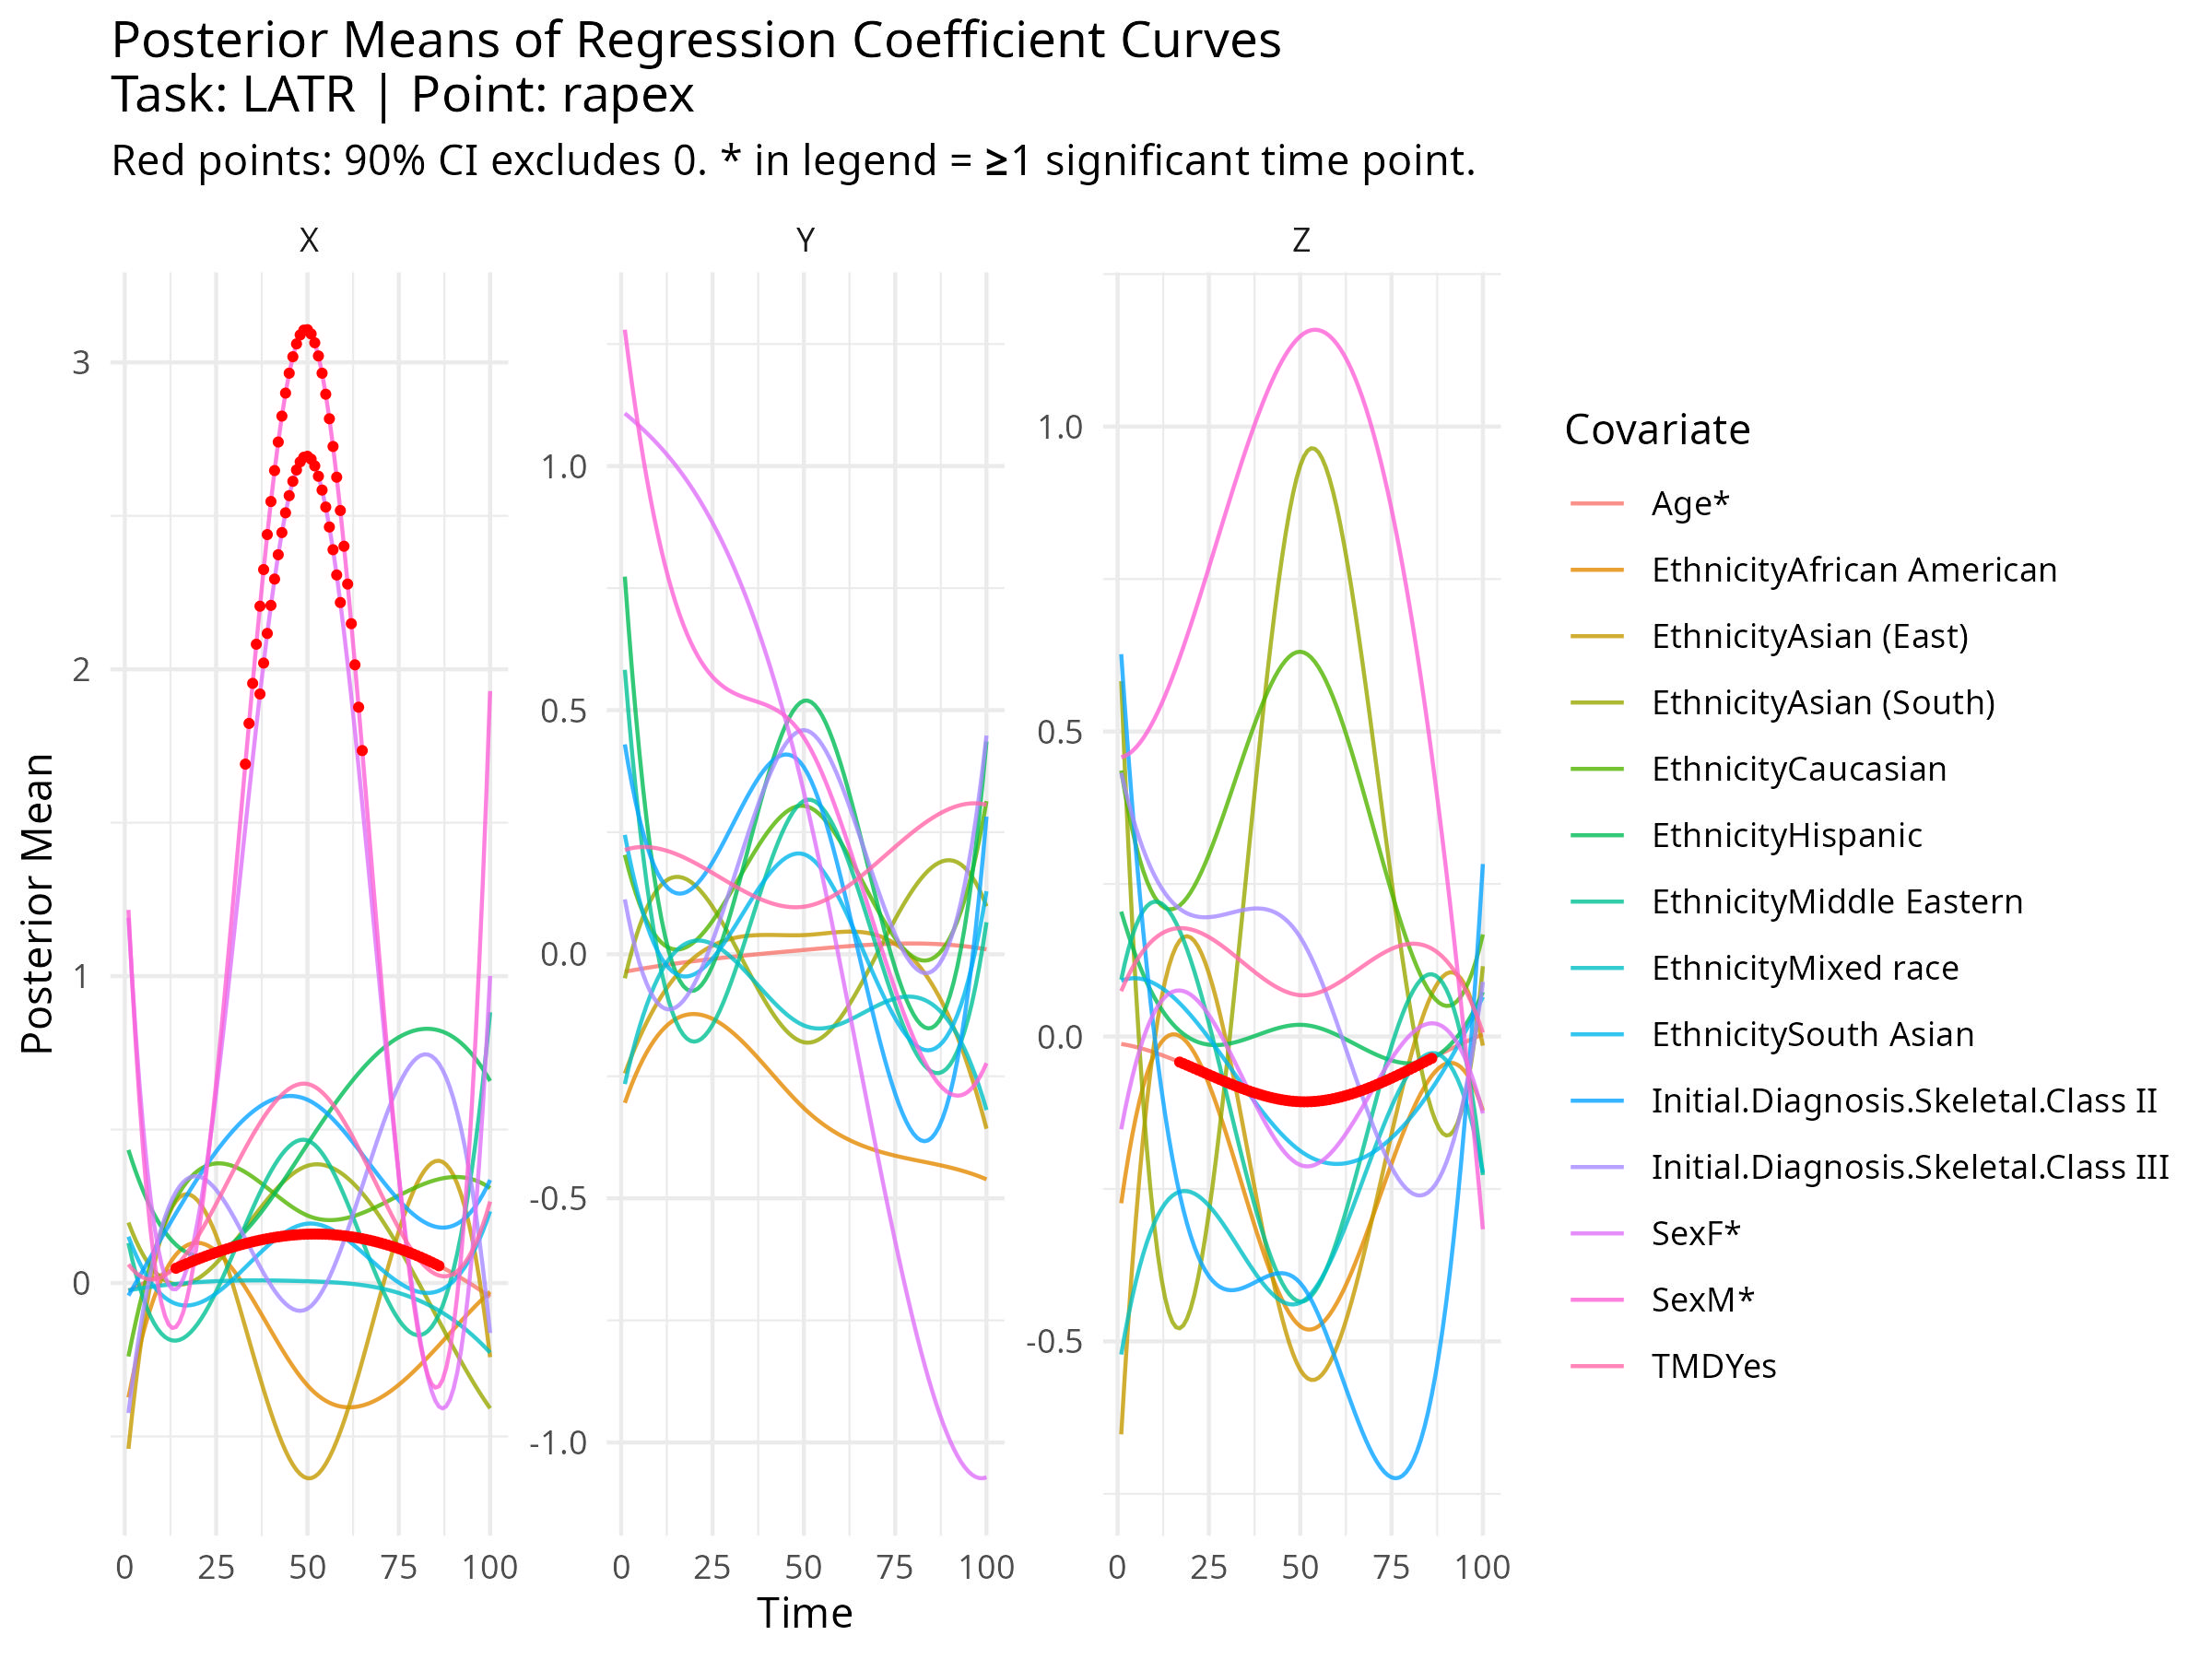
\includegraphics[width = 0.7\textwidth]{latR_rapex_plot.jpeg}
    \caption{Results for Lateral Right Task, Right Apex tracking point.}
    \label{fig:latR_rapex}
\end{figure}

\begin{figure}[h]
    \centering
    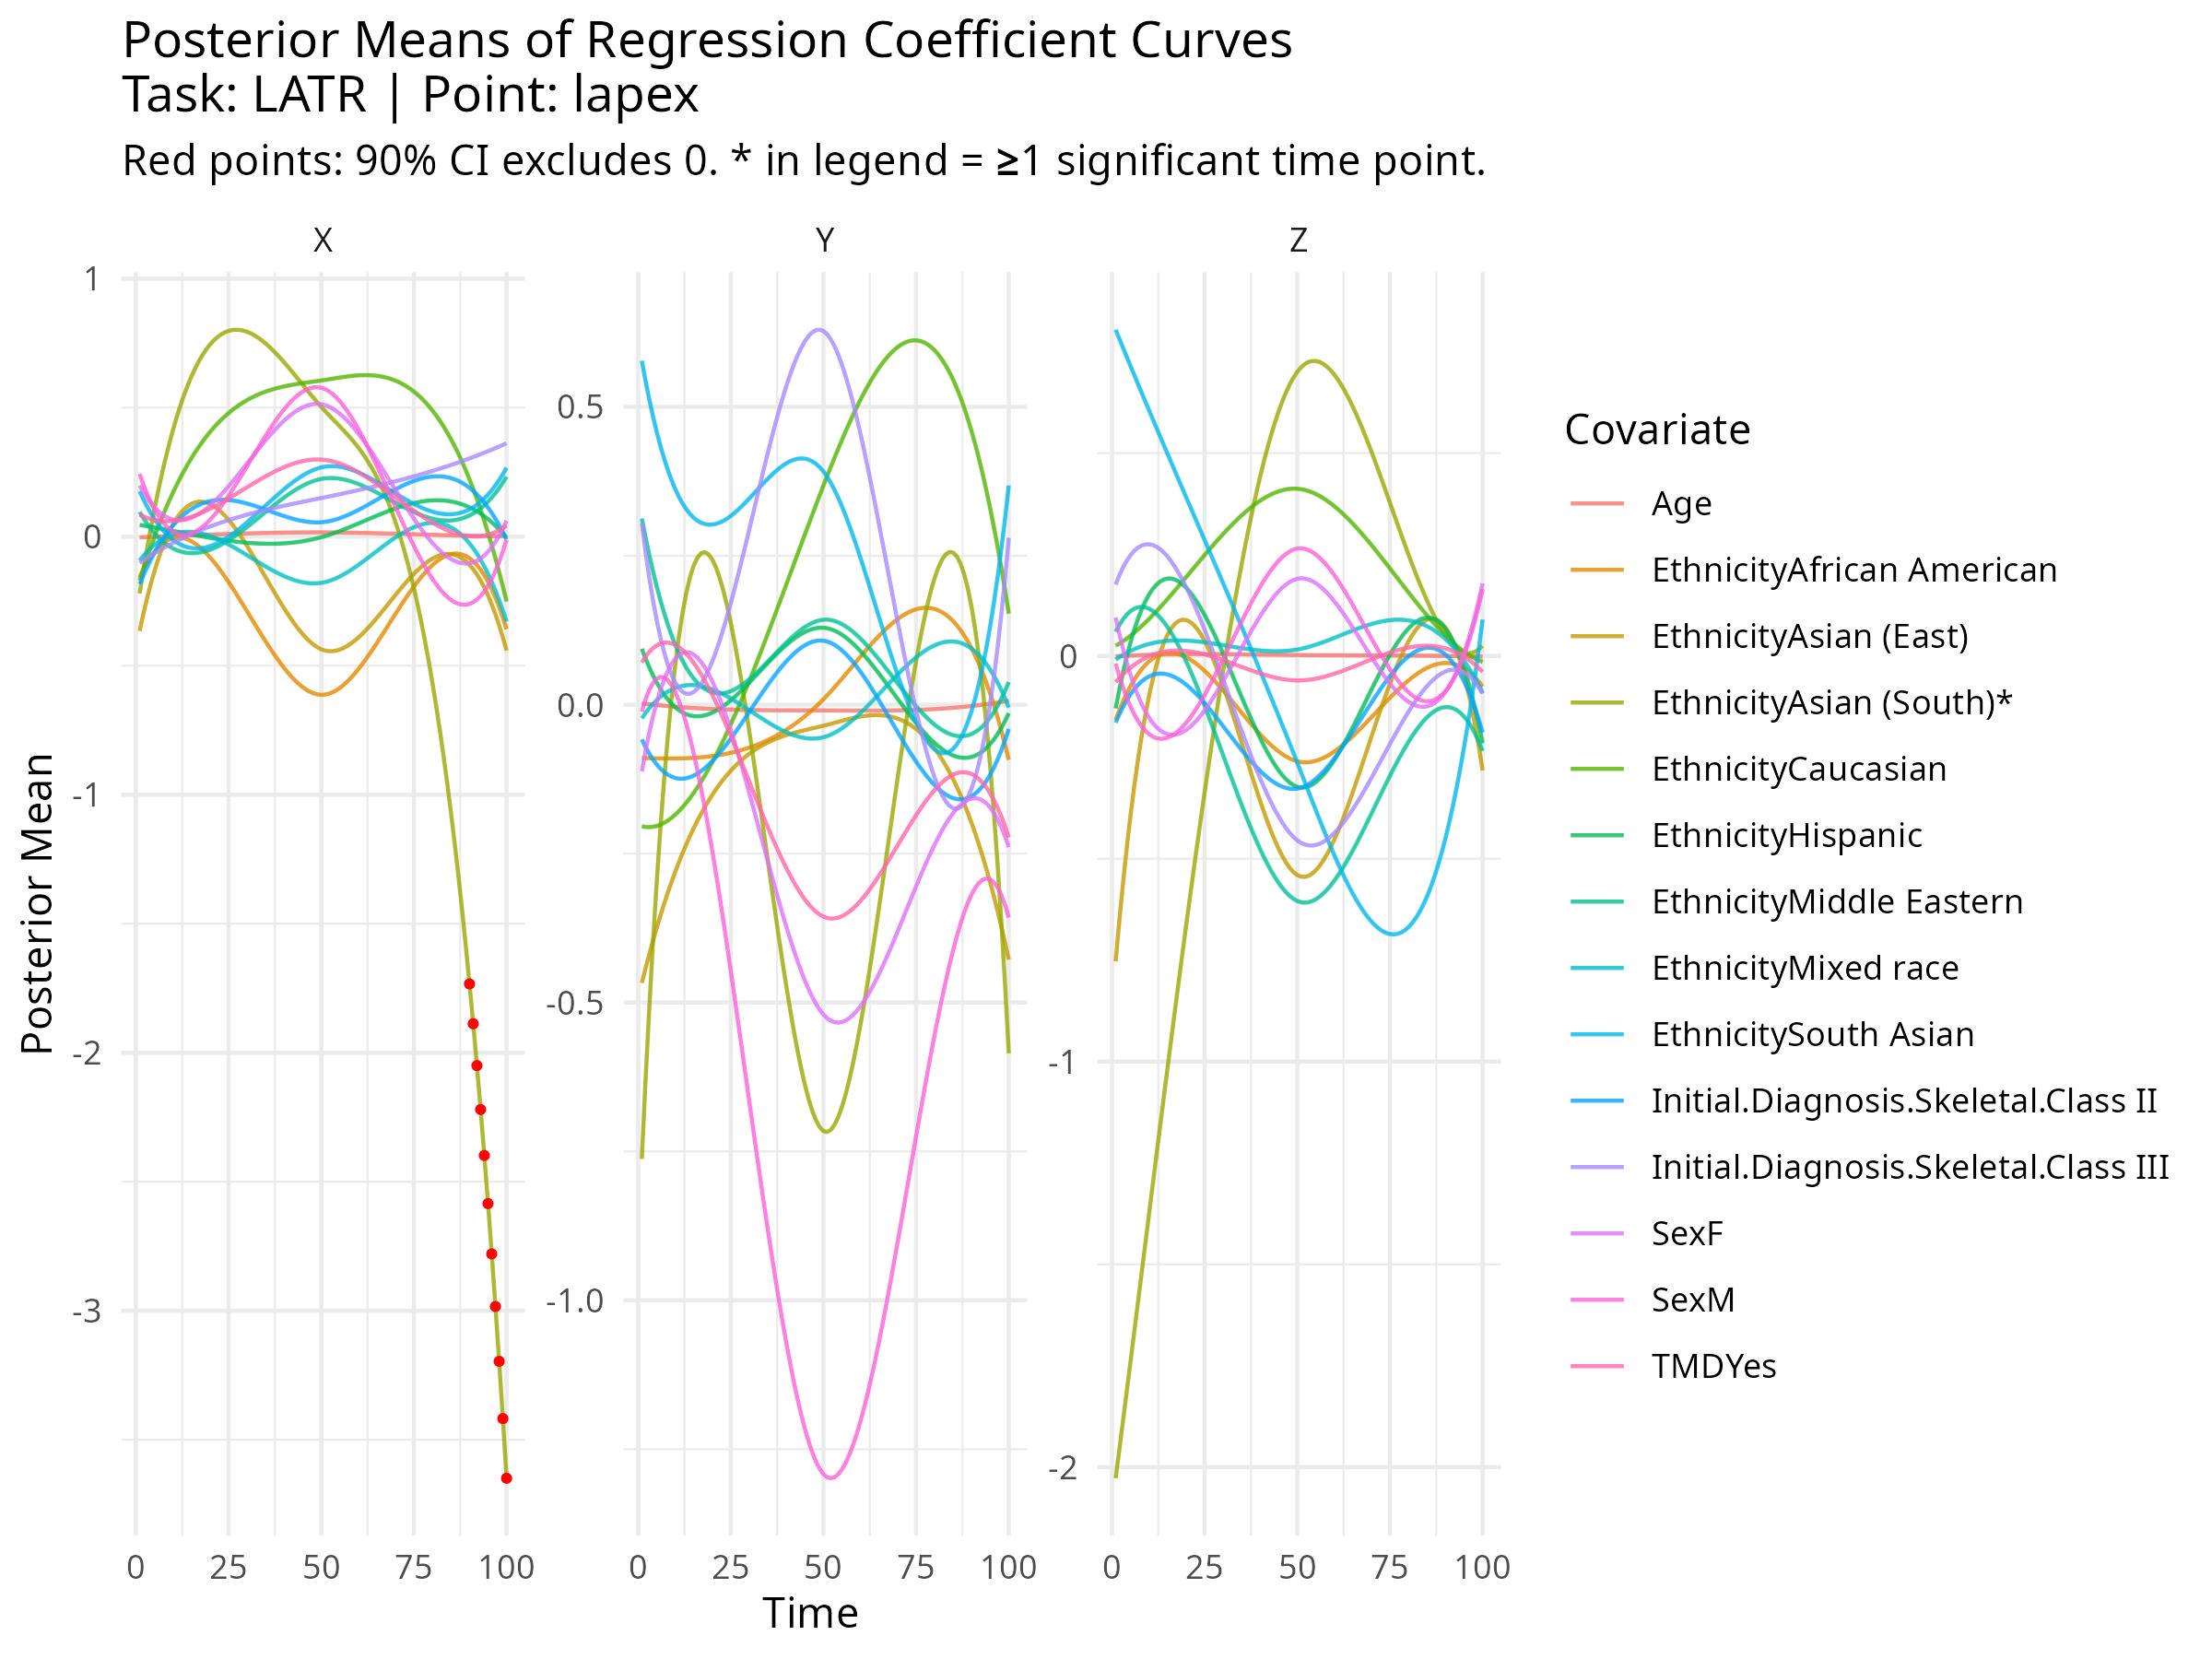
\includegraphics[width = 0.7\textwidth]{latR_lapex_plot.jpeg}
    \caption{Results for Lateral Right Task, Left Apex tracking point.}
    \label{fig:latR_lapex}
\end{figure}

\begin{figure}[h]
    \centering
    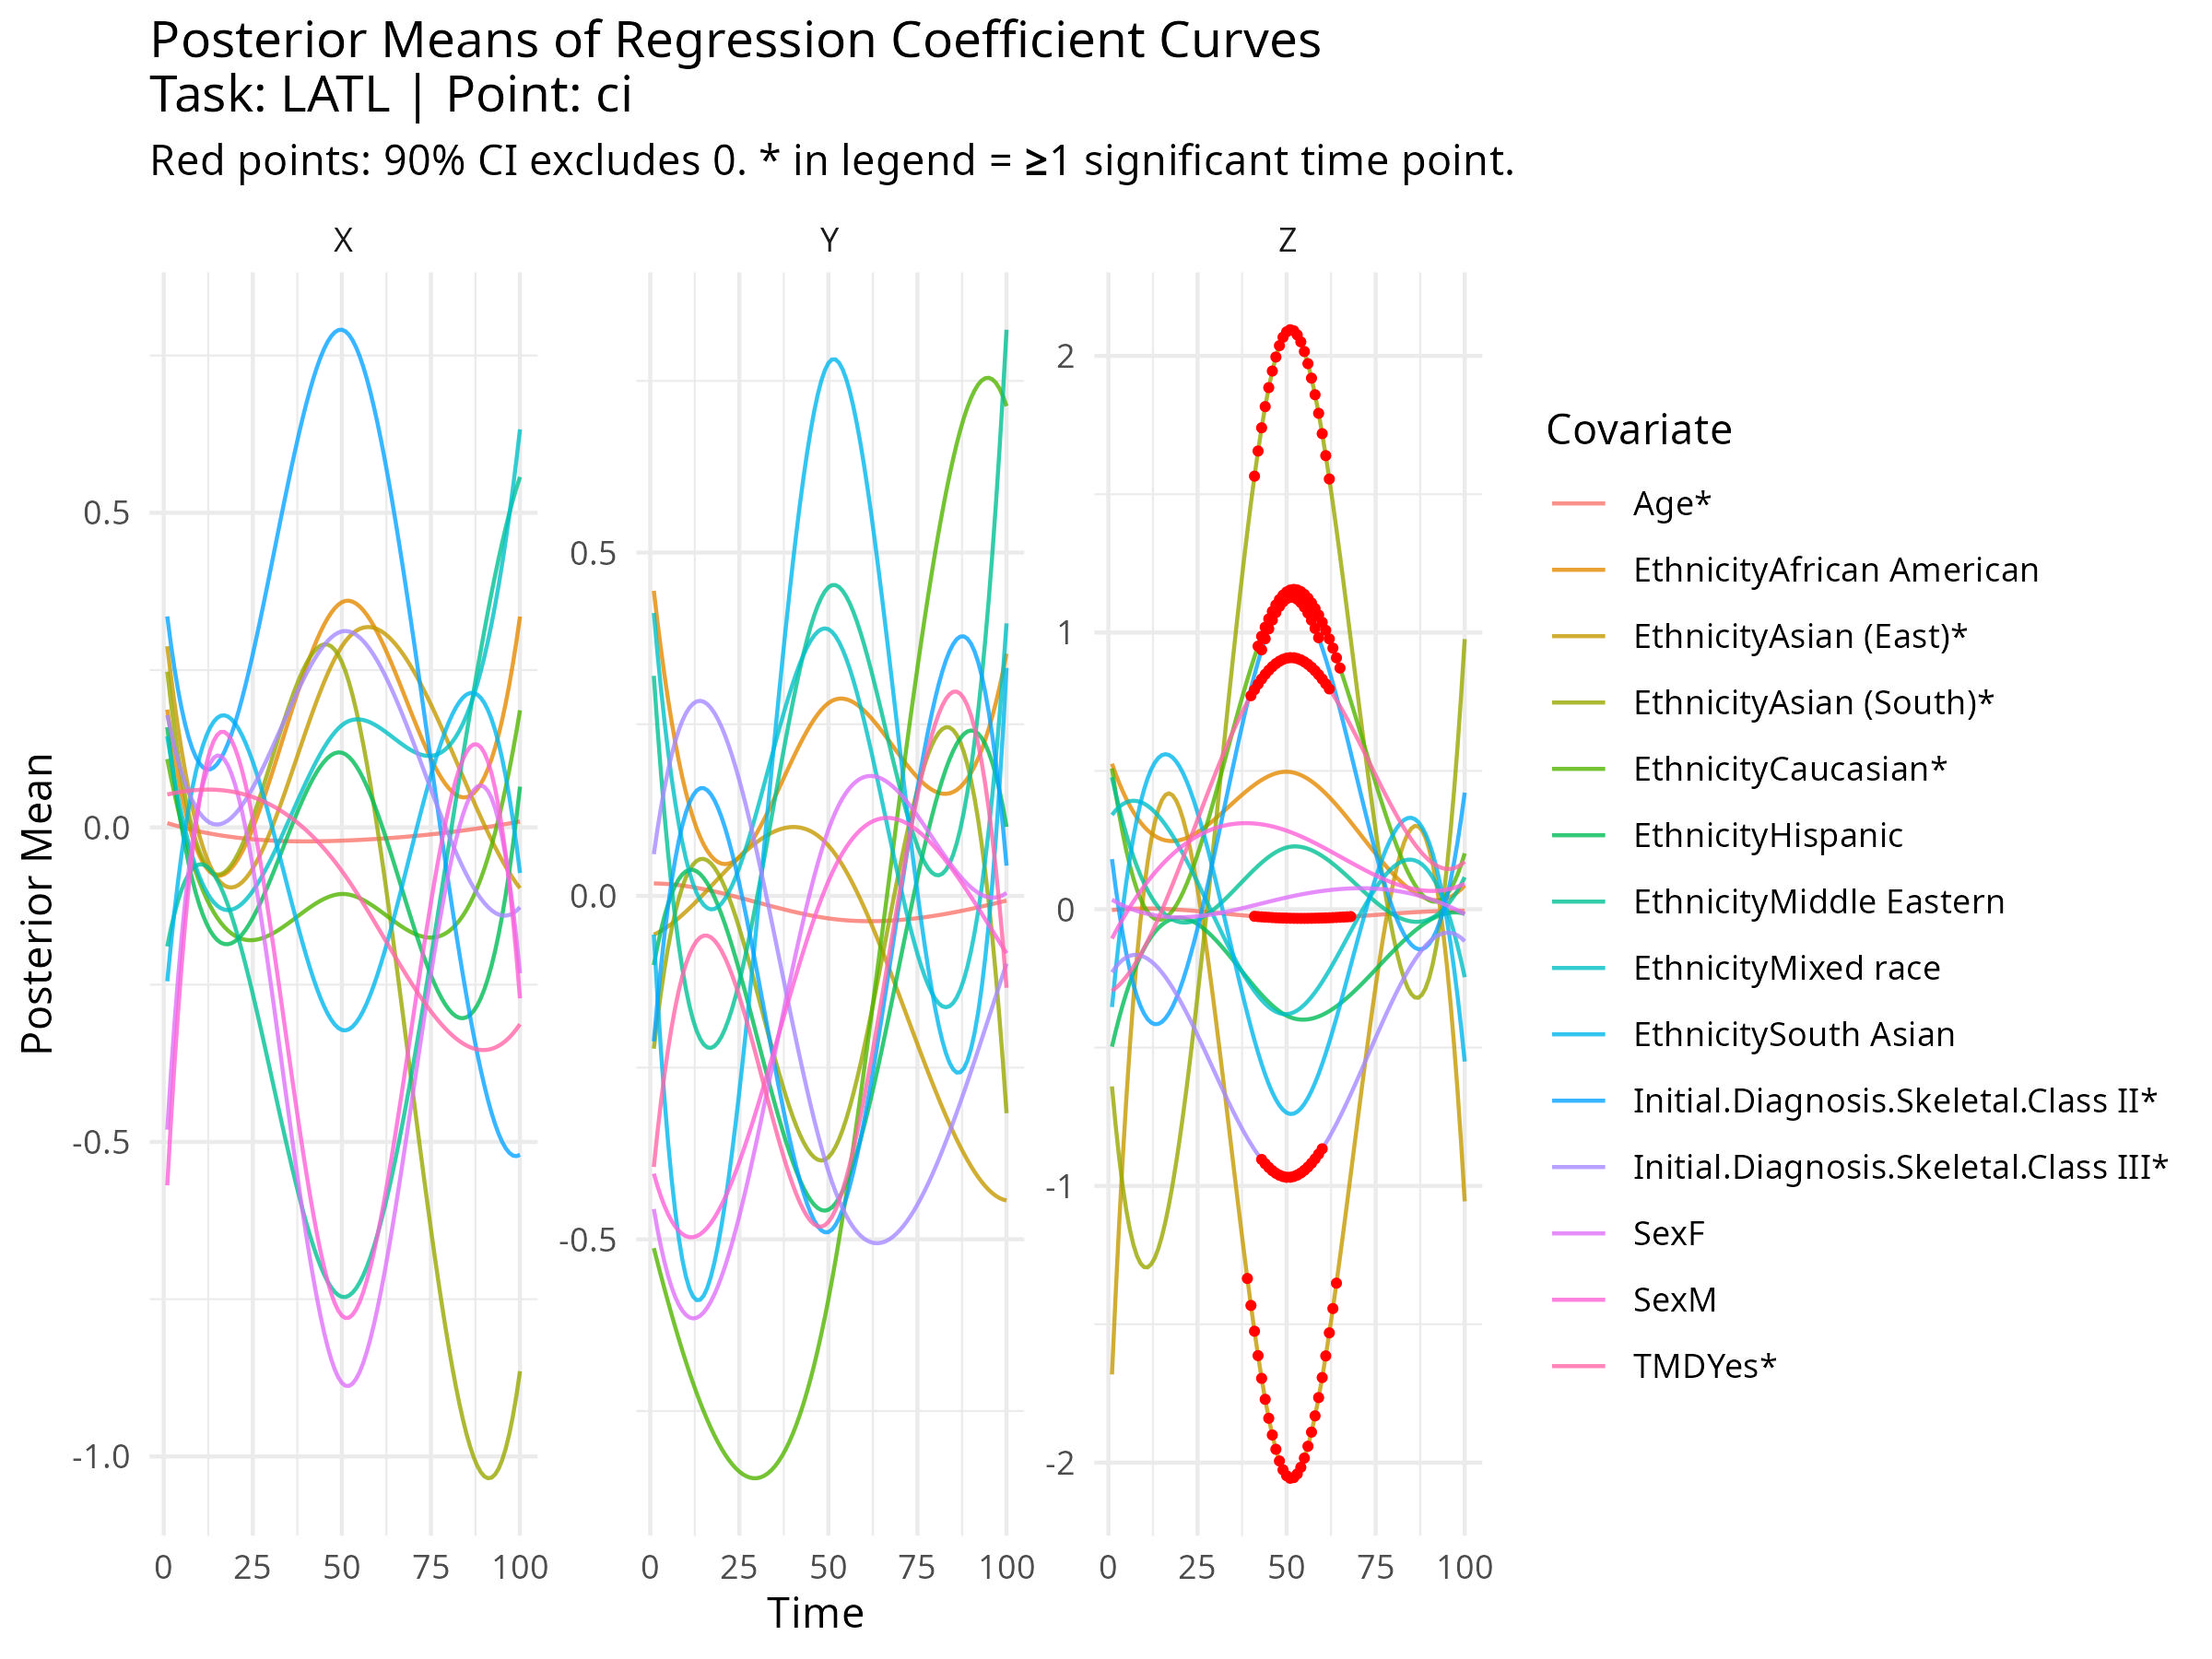
\includegraphics[width = 0.7\textwidth]{latL_ci_plot.jpeg}
    \caption{Results for Lateral Left Task, Central Incisor tracking point.}
    \label{fig:latL_ci}
\end{figure}

\begin{figure}[h]
    \centering
    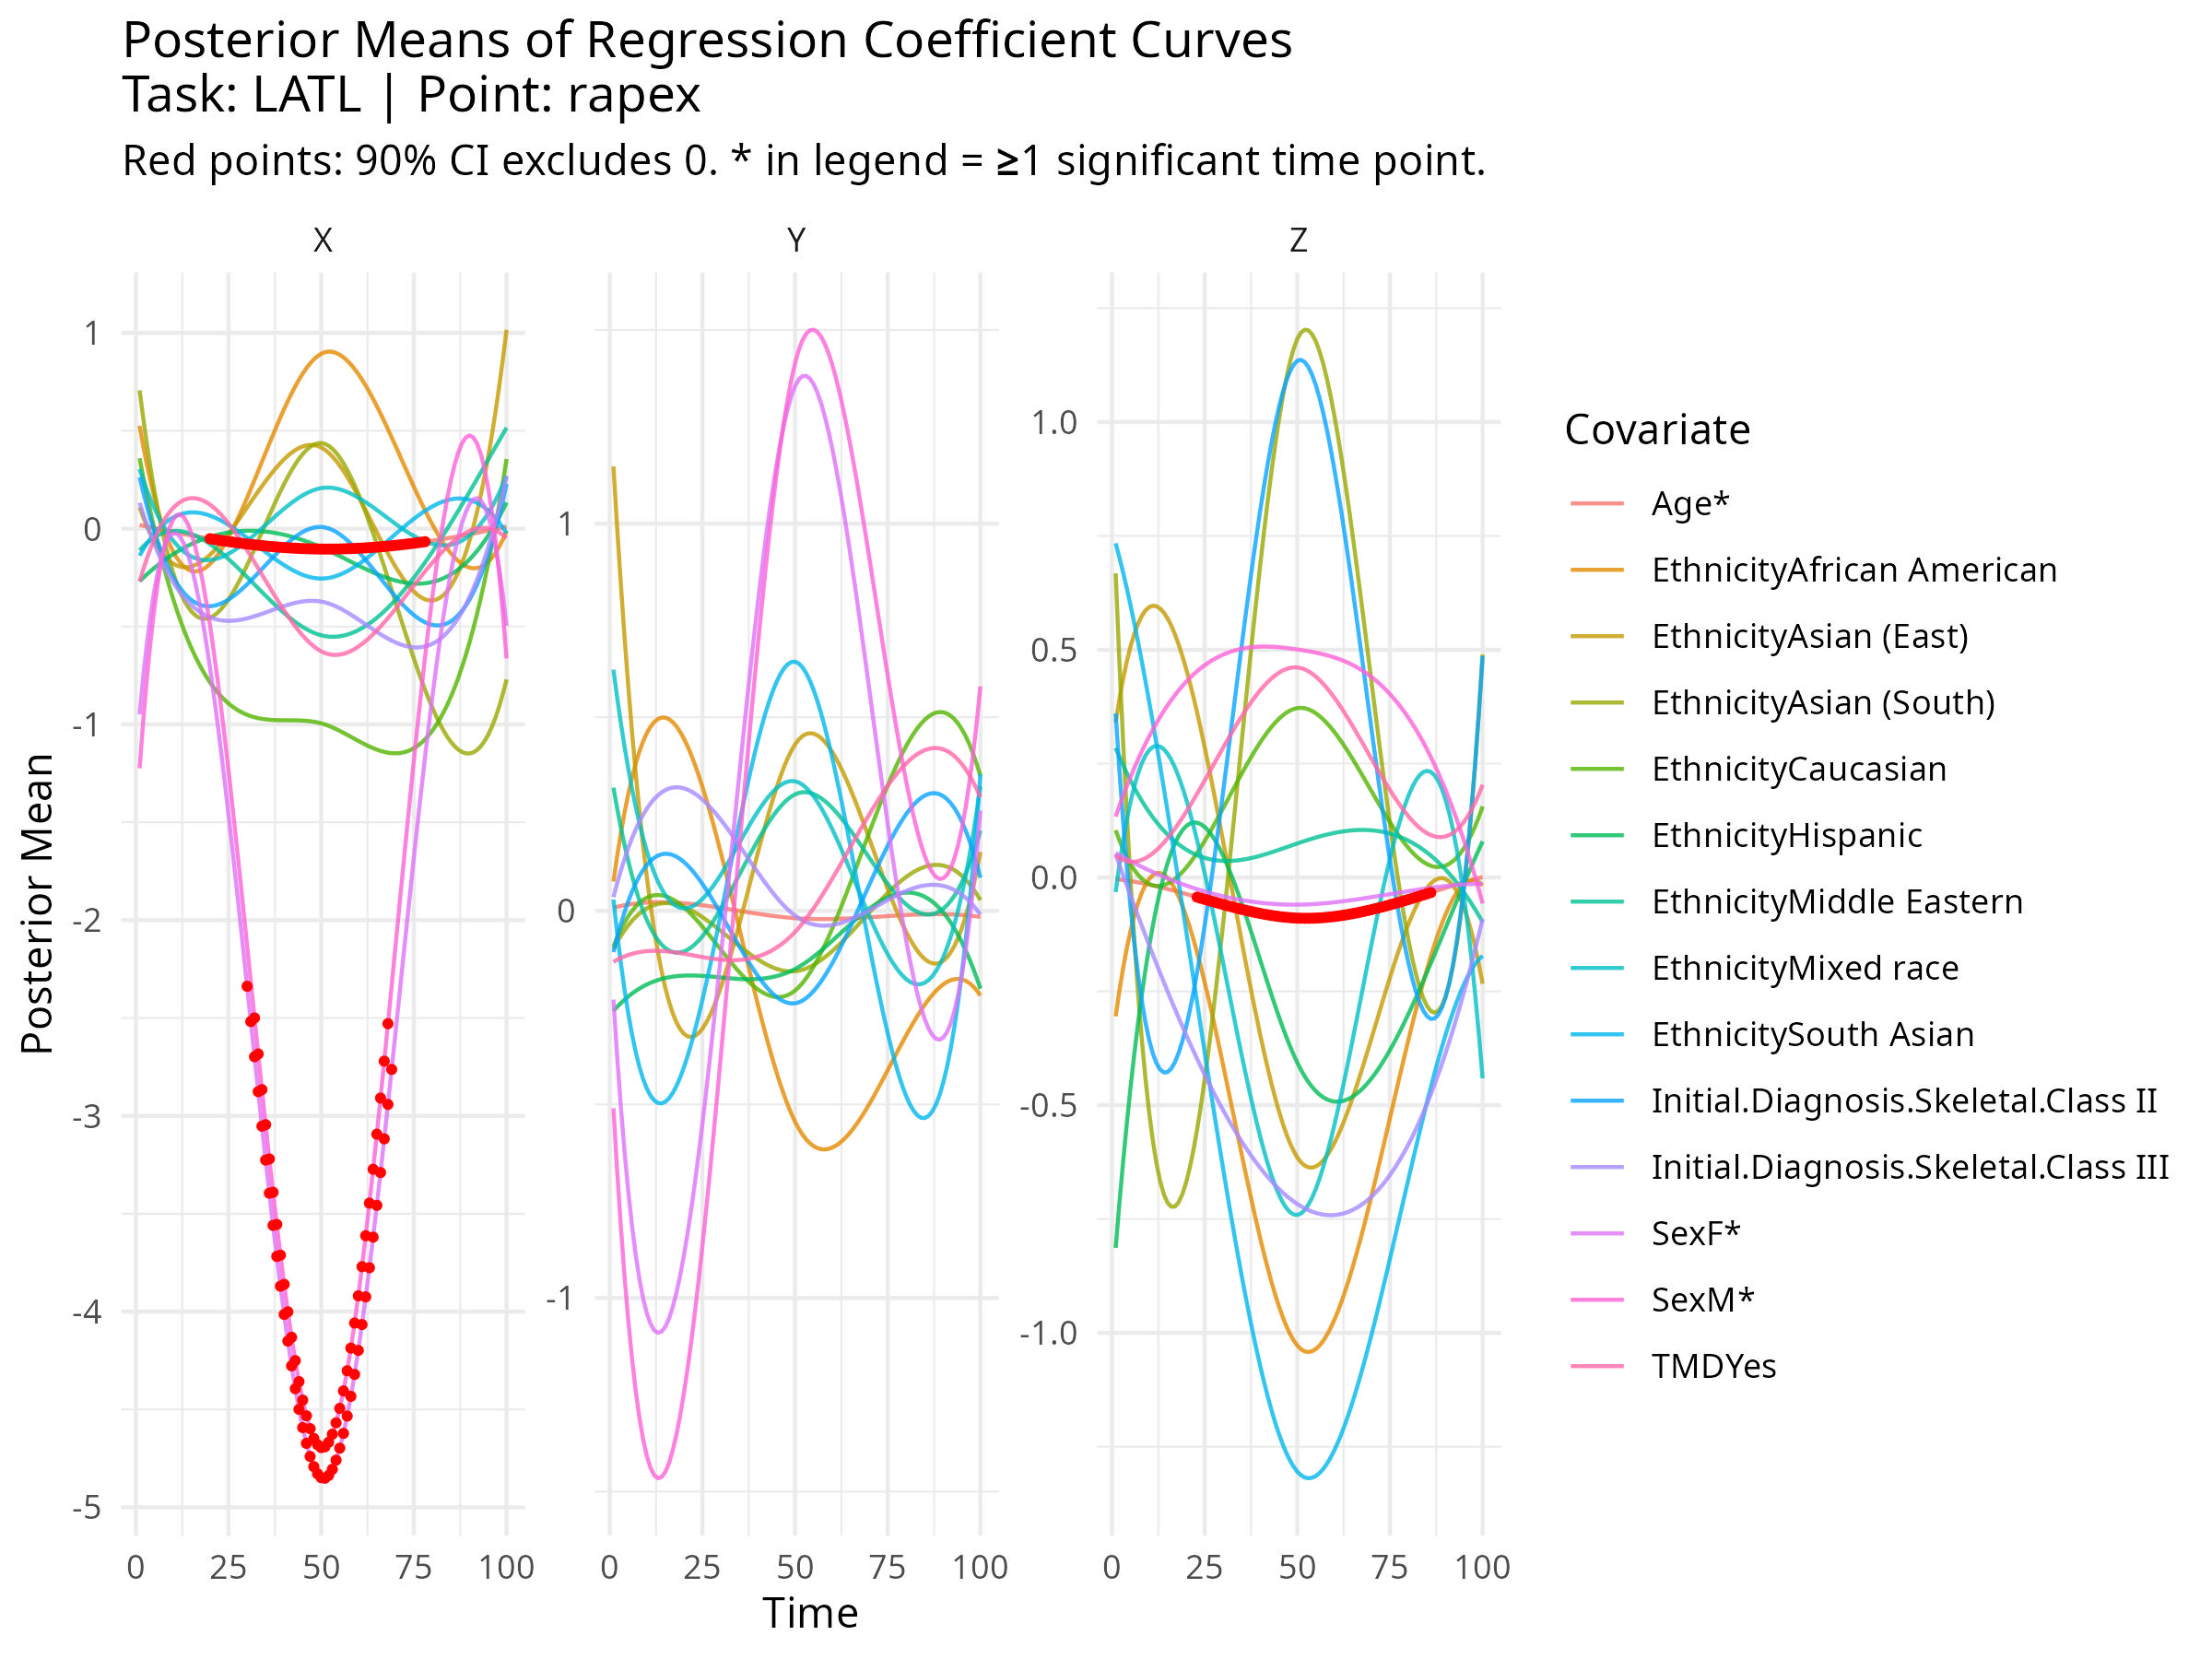
\includegraphics[width = 0.7\textwidth]{latL_rapex_plot.jpeg}
    \caption{Results for Lateral Left Task, Right Apex tracking point.}
    \label{fig:latL_rapex}
\end{figure}

\begin{figure}[h]
    \centering
    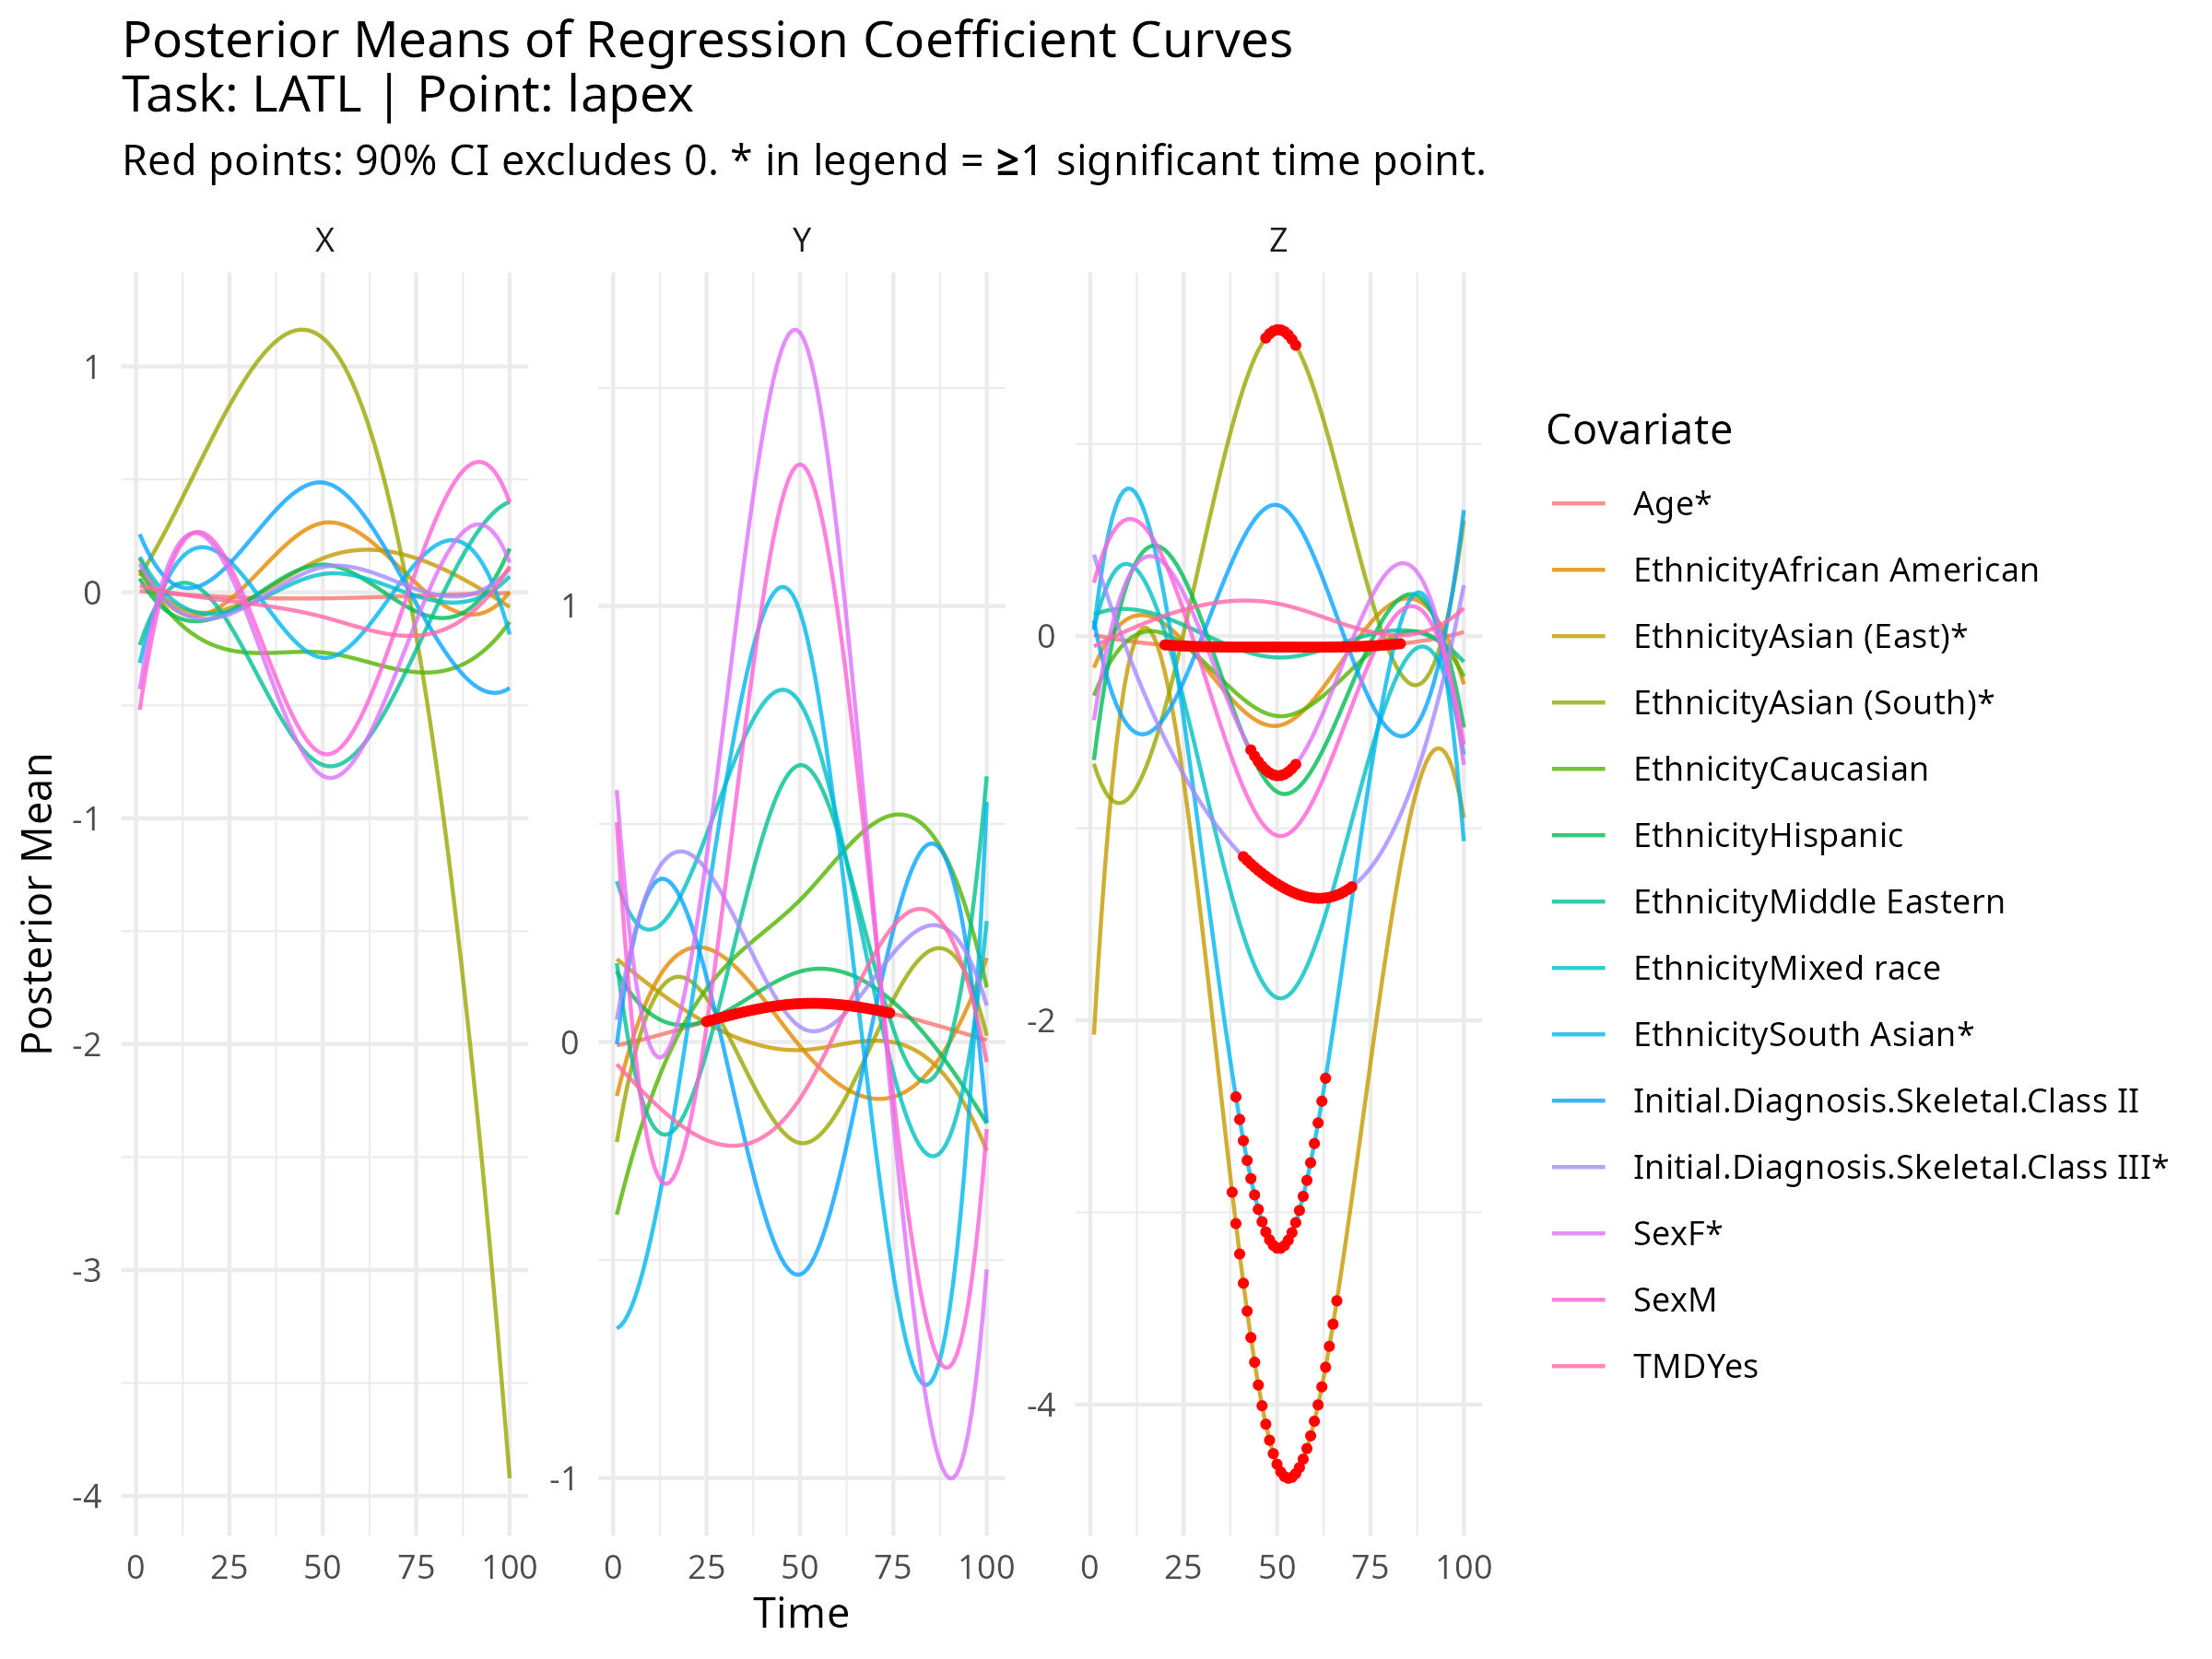
\includegraphics[width = 0.7\textwidth]{latL_lapex_plot.jpeg}
    \caption{Results for Lateral Left Task, Left Apex tracking point.}
    \label{fig:latL_lapex}
\end{figure}

\nocite{*}% Show all bib entries - both cited and uncited; comment this line to view only cited bib entries;


%\bmsection*{Author Biography}

%\begin{biography}{
\includegraphics[width=76pt,height=76pt,draft]{empty}}{
%{\textbf{Author Name.} Please check with the journal's author guidelines whether
%author biographies are required. They are usually only included for
%review-type articles, and typically require photos and brief
%biographies for each author.}}
%\end{biography}


\end{document}
